% @Author: Mouna REKIK
% @Date:   2024-10-11 / 12:30
%%%%%%%%%%%%%%%%%%%%%%%%%%%%%%%%%%%%%%%%%%%%%%%%%%%%%%%%%%%%%%%%%%%%%%%%%%%%%%

\chapter{Réalisation et évaluation}
\begin{spacing}{1.2}
\minitoc
\thispagestyle{MyStyle}
\end{spacing}
\newpage

\section{Introduction}
Ce chapitre présente la concrétisation de la plateforme conçue dans le chapitre précédent. 
L’objectif est de montrer comment l’architecture pensée a été traduite en un système opérationnel, 
en décrivant son déploiement, son fonctionnement interne et son utilisation pratique. 
Nous illustrons ces étapes à l’aide de captures d’écran, d’extraits de code et de scénarios d’utilisation.

\section{Mise en place de l’environnement}
La plateforme a été déployée sur Microsoft Azure en exploitant les services présentés précédemment.
Les microservices ont été conteneurisés avec Docker et orchestrés à l’aide de \texttt{docker-compose}. 
Avant de présenter les \textit{endpoints} exposés, nous décrivons la configuration des services Azure utilisés dans la solution.

\subsection{Déploiement des modèles}
Les modèles de langage (LLMs) ont été déployés en fonction des besoins spécifiques de chaque agent. 
Ainsi, les modèles \texttt{gpt-5-mini} et \texttt{gpt-5-nano} ont été disponibles seulement dans la région \textit{East-US}.
\begin{figure}[H]%
\centering
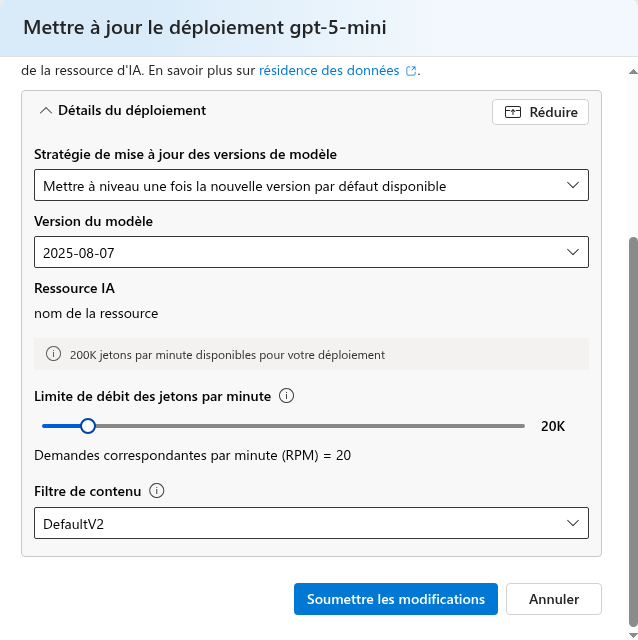
\includegraphics[keepaspectratio,height=7cm]
{images/param_deploy.png}%
\caption{Paramétrage de déploiement du modèle}%
\label{fig:param_deploy}
\end{figure}
Comme illustré dans la  \ref{fig:param_deploy}, nous configurons les paramètres du déploiement, tels que la limite de jetons par minute.
De même, le modèle d’embeddings \texttt{text-embedding-3-small} ainsi que les LLMs \texttt{gpt-4} et \texttt{gpt-4o-mini} ont été déployés dans la région \textit{West-US}.
\begin{figure}[H]%
\centering
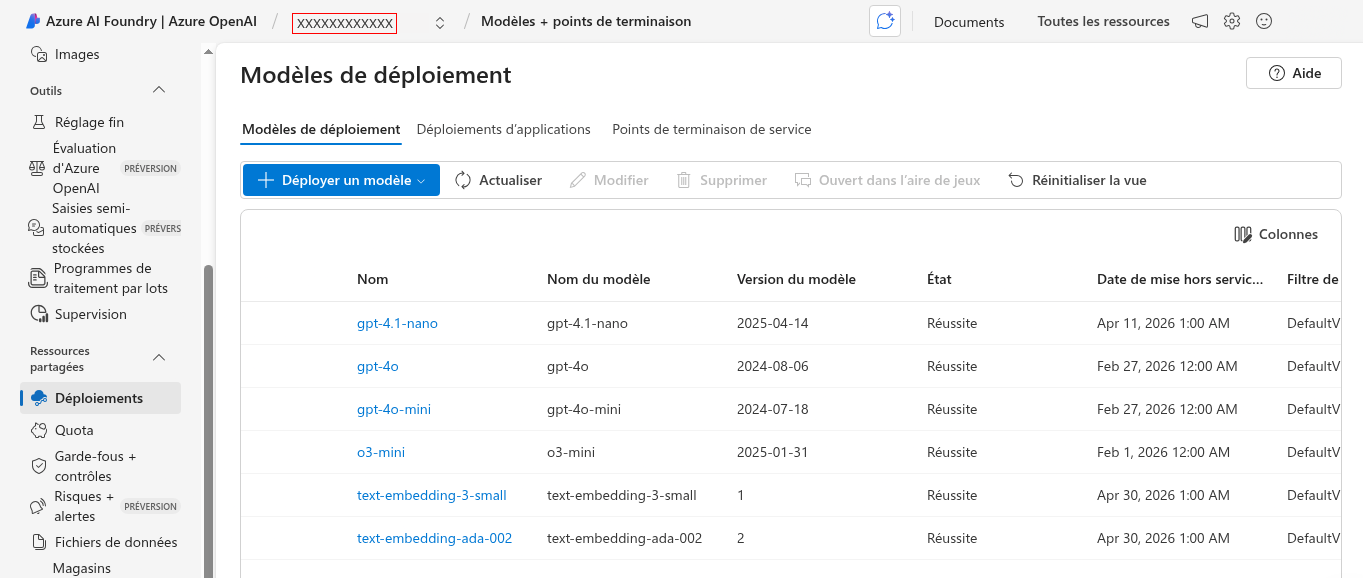
\includegraphics[keepaspectratio,height=6cm]
{images/list_deploy_.png}%
\caption{Liste des déploiements}%
\label{fig:list_deploy}
\end{figure}
Chaque ensemble de déploiements appartient à une ressource. D'après la figure \ref{fig:list_deploy} Azure assigne chaque ressource à un groupe de ressources et une souscription. Nous remarquons que chaque ressource possède ainsi sa région où elle est créée, son point de terminaison (endpoint) et sa clé pour pouvoir les utiliser par nos microservices concernés.
\begin{figure}[H]%
\centering
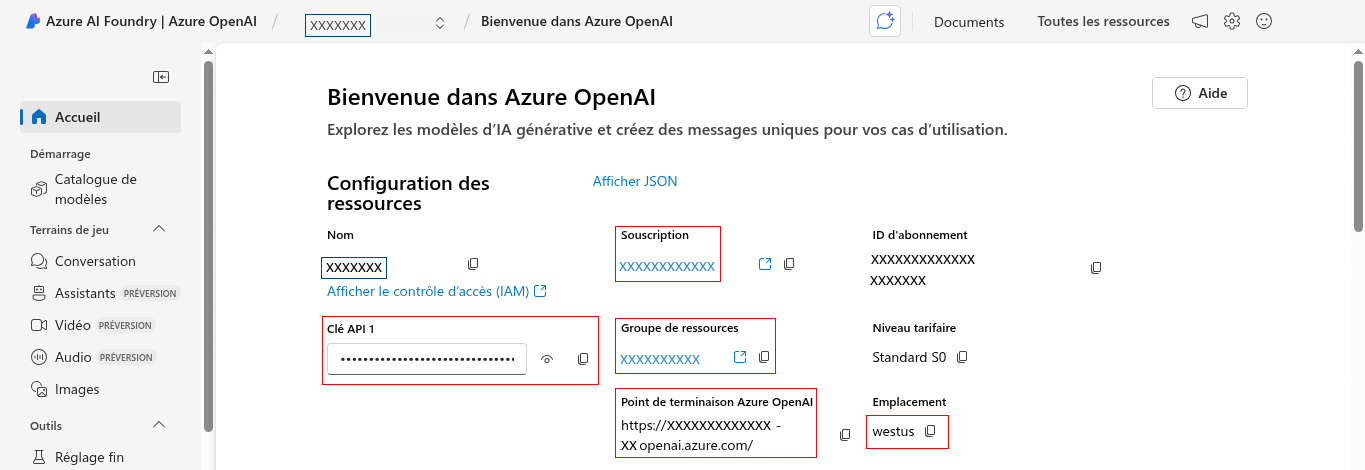
\includegraphics[keepaspectratio,width=\textwidth]
{images/config_.png}%
\caption{Configuration d'une ressource openai}%
\label{fig:config}
\end{figure}
La section \textit{Metrics} d’Azure permet de visualiser la consommation des jetons de chaque déploiement, et ainsi d’optimiser l’utilisation et les coûts. La figure \ref{fig:mesure} montre bien les statistiques d'utilisation avec des métriques comme le nombre total de requêtes, le nombre de jetons par prompt (input), génère par le modèle (output) et total. En cas de mise en production, cette section devient inutile et nous devrons mettre des alertes et des limites grâce au service Azure monitor.
\begin{figure}[H]%
\centering
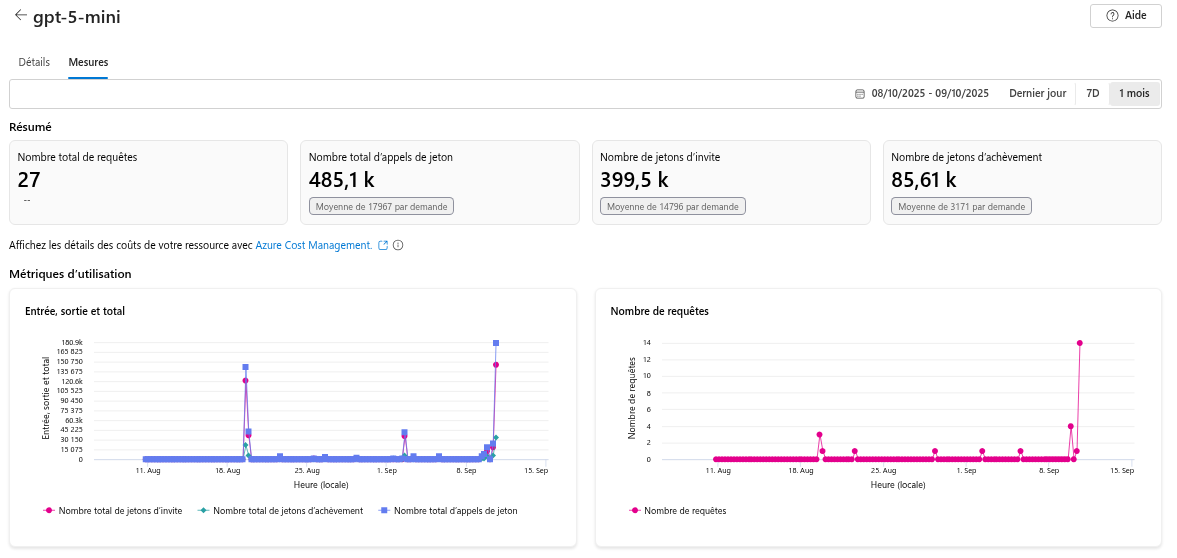
\includegraphics[keepaspectratio,height=6cm]
{images/mesure.png}%
\caption{Dashboard des mesures d'un déploiement}%
\label{fig:mesure}
\end{figure}
La plateforme d'Azure AI Foundry permet non seulement de consommer un modèle à travers une API, mais aussi de le tester à travers une section de discussions en définissant les instructions et les paramètres nécessaires.
\begin{figure}[H]%
\centering
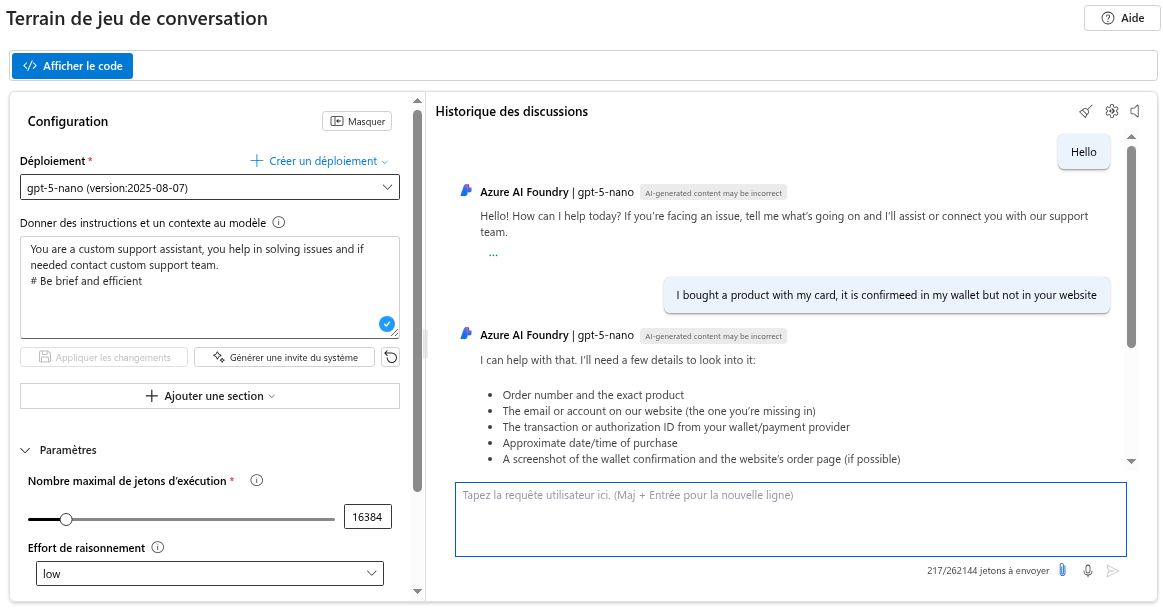
\includegraphics[keepaspectratio,height=6cm]
{images/chat_azure_.png}%
\caption{Dashboard des mesures d'un déploiement}%
\label{fig:chat_azure}
\end{figure}

\subsection{Préparation des sources de données}
Deux sources principales ont été exploitées : \textit{Azure Blob Storage} et \textit{Azure SQL Database}.
\begin{figure}[H]%
\centering
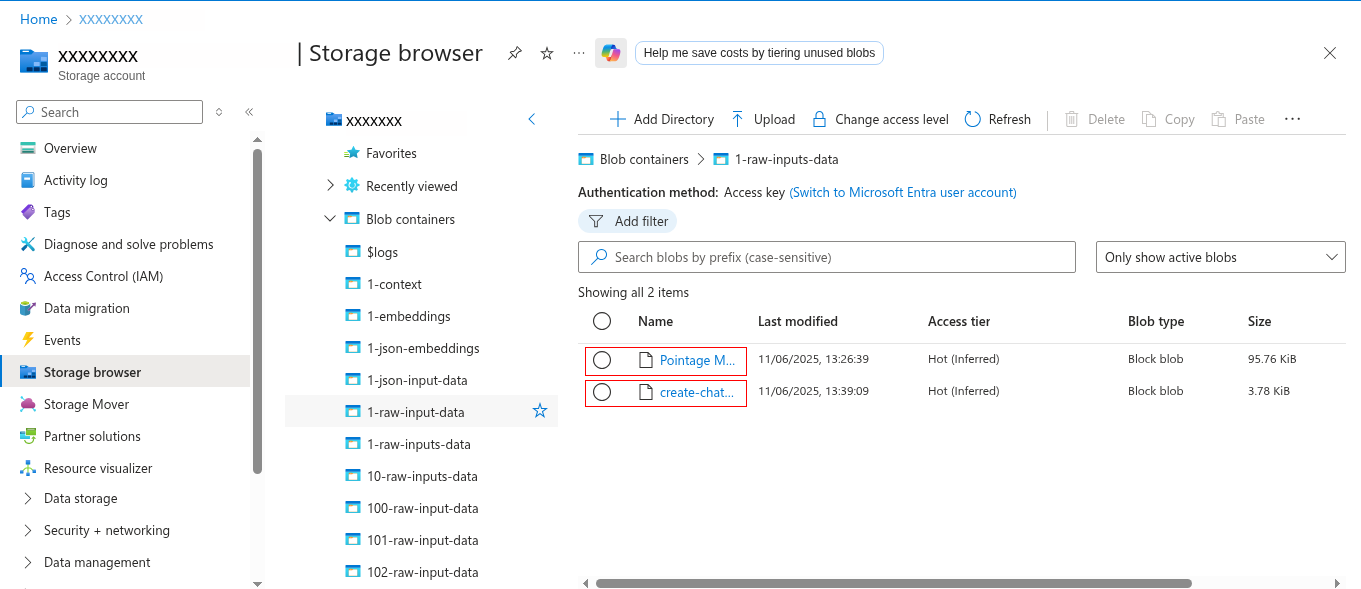
\includegraphics[keepaspectratio,height=6cm]
{images/blob_.png}%
\caption{Conteneurs Blob chez Azure}%
\label{fig:blob}
\end{figure}
La figure \ref{fig:blob} illustre la séparation des conteneurs Blob, nommés de manière à correspondre à chaque chatbot. 
Chaque conteneur contient plusieurs \textit{block blobs}, chacun correspondant à un fichier chargé par l’utilisateur pour un assistant. 
Ces fichiers constituent la base de connaissances exploitée par le mécanisme \textit{Retrieval Augmented Generation} (RAG).  
Les \textit{block blobs} stockent du texte et des données binaires. Ils sont constitués de blocs pouvant être gérés individuellement et peuvent contenir jusqu’à 190,7~TiB de données.

Une ressource \textit{SQL Database} a été allouée, comprenant les tables nécessaires au fonctionnement de la plateforme.
\begin{figure}[H]%
\centering
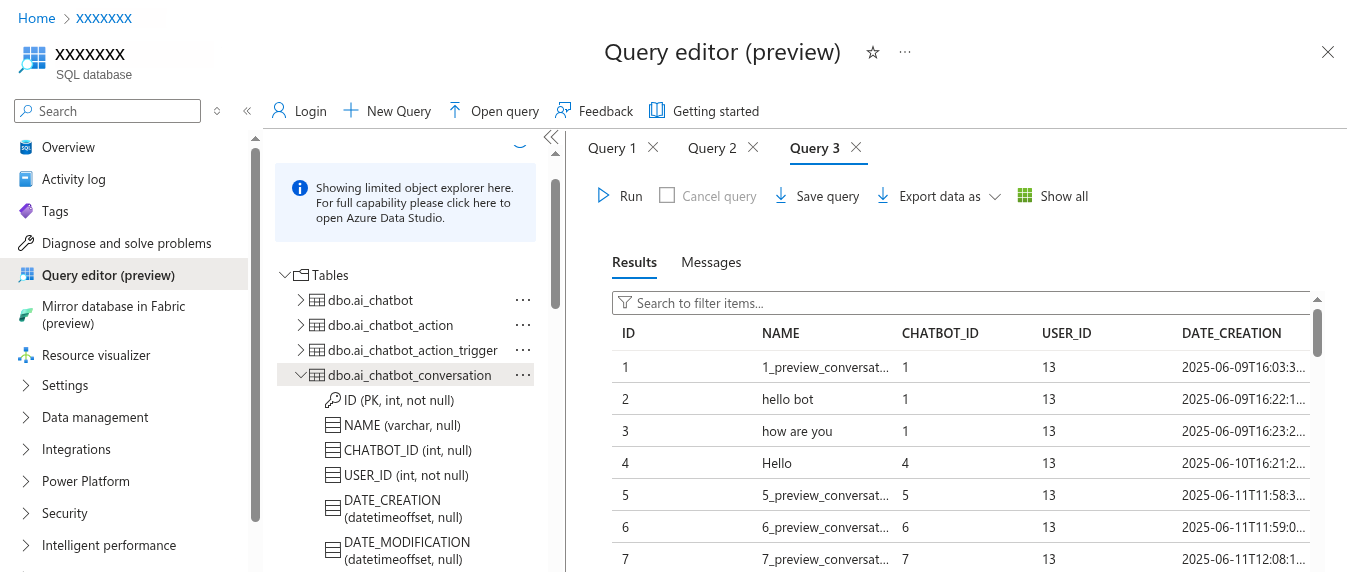
\includegraphics[keepaspectratio,width=\textwidth]
{images/sql.png}%
\caption{Base de données SQL chez Azure}%
\label{fig:sql}
\end{figure}
Les entités stockées respectent les bonnes pratiques, incluant notamment des colonnes de création et de suppression afin de garantir une traçabilité complète.

\section{Choix technologiques}
La sélection des technologies pour notre plateforme a été guidée par les exigences de flexibilité et d'intégration fluide avec des outils d'IA, en alignement direct avec l'objectif de développer une solution permettant la gestion personnalisée de chatbots, avec une base de connaissances dynamique et des actions configurables sans code. Ces choix facilitent le développement rapide, la maintenance et l'adaptabilité aux besoins des administrateurs et utilisateurs finaux, en optimisant les flux conversationnels et en minimisant les temps de réponse
\subsection{Langage backend}
Python \cite{python-docs} a été choisi comme langage central pour le backend en raison de son écosystème riche et de son support étendu pour les bibliothèques d'intelligence artificielle et de RAG, telles que LangChain, LlamaIndex, Hugging Face, OpenAI... Ce langage offre une interopérabilité simple avec la majorité des frameworks agentiques existants, permettant une intégration rapide des modèles d'IA avancés nécessaires pour les chatbots personnalisés. De plus, Python est particulièrement facile à développer, avec une syntaxe claire et concise qui accélère le prototypage et les itérations, tout en étant ouvert et adapté aux manipulations de données complexes – essentielles pour indexer des fichiers variés et gérer des sources dynamiques comme des URLs en temps réel. Dans le cadre de notre projet, cette facilité a permis de concentrer les efforts sur la personnalisation des assistants virtuels, en rendant le traitement des bases de connaissances et des actions plus efficace, contribuant ainsi à l'objectif d'une plateforme adaptable aux domaines d'activité spécifiques.


\subsection{Outils de développement et de test}
Pour soutenir un développement efficace et rigoureux, plusieurs outils ont été adoptés, chacun jouant un rôle clé dans la réalisation de notre objectif.
\subsubsection{VSCode}
Visual Studio Code \cite{vscode-docs} (VSCode) sert d'IDE principal, enrichi d'extensions dédiées à Python, Docker et Git, facilitant un environnement de codage intégré et productif. Cet outil accélère le développement des microservices et des agents, permettant de tester rapidement les interactions conversationnelles et d'assurer une compatibilité avec les services Azure.
\subsubsection{Postman}
Postman \cite{postman-docs} a été utilisé pour tester et valider les APIs exposées par les microservices, en simulant divers scénarios de requêtes et de réponses, ce qui est crucial pour vérifier la fluidité des échanges entre le frontend et l'orchestrateur, garantissant ainsi une expérience utilisateur sans faille lors de la configuration ou de l'utilisation des chatbots.
\subsubsection{Git}
Git \cite{git-docs} gère le code source et le suivi des versions, avec une organisation en branches adaptée aux environnements de développement, test et production. Intégré à \textbf{Azure Repos}, cet outil renforce la collaboration et la traçabilité, permettant une gestion agile des évolutions de la plateforme et une intégration continue des nouvelles fonctionnalités.
\subsubsection{LangSmith}
LangSmith \cite{langsmith-docs}, outil d’observabilité proposé par LangChain, permet de monitorer, déboguer et évaluer les performances des agents et des chaînes, offrant une visibilité détaillée sur les flux agentiques. Dans notre contexte, cela assure une réduction des hallucinations et une optimisation des prompts, alignée sur l'objectif de réponses précises et contextualisées.
\subsubsection{LangGraph Studio}
LangGraph Studio \cite{langchain-studio-docs} fournit un environnement pour expérimenter, prototyper et tester rapidement des graphes et des agents, facilitant l'itération sur les architectures multi-agents et accélérant le développement de chatbots adaptés aux besoins spécifiques des utilisateurs finaux.
\begin{figure}[H]%
\centering
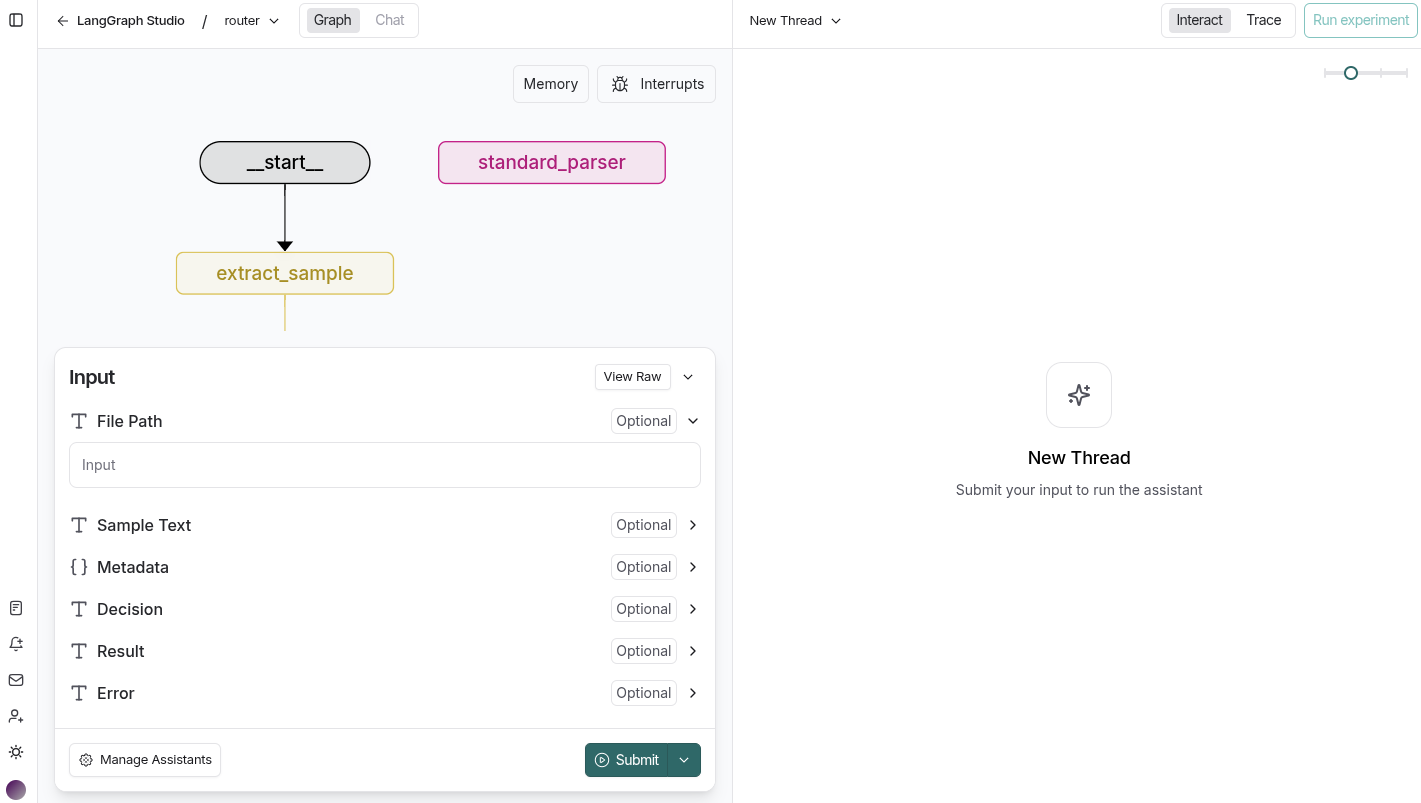
\includegraphics[keepaspectratio,width=\textwidth]
{images/langgraph_studio.png}%
\caption{Langgraph studio}%
\label{fig:studio}
\end{figure}
L'interface est très efficace avec la possibilité de voir l'architecture et les exécutions, de modifier librement les entrées et sorties du système.

\subsubsection{Conteneurisation et orchestration}
Docker \cite{docker-docs} a été employé pour conteneuriser chaque microservice, assurant la portabilité, la scalabilité et une isolation optimale des composants. Cette approche simplifie les déploiements sur Azure et facilite la gestion des dépendances, comme l'intégration avec Azure OpenAI Service ou les bases vectorielles. Dans le cadre de notre projet, Docker contribue à l'objectif de modularité en permettant une communication vive des microservices (frontend, orchestrateur, gestion, RAG), tout en supportant une scalabilité horizontale pour gérer un nombre croissant de chatbots personnalisés sans compromettre les performances.

\subsubsection{Gestion de projet et suivi}
Azure Boards \cite{azure-boards-docs} a été adopté comme outil de gestion agile (Kanban/Scrum), permettant de planifier, suivre et prioriser les tâches de développement. Son intégration avec Git facilite la traçabilité des commits et des user stories, assurant une collaboration fluide au sein de l'équipe. Dans notre projet, cet outil a joué un rôle essentiel pour aligner les itérations de développement sur l'objectif global, en gérant efficacement les phases de conception des agents, d'intégration des bases de connaissances et de test des actions configurables, garantissant ainsi une livraison continue d'une plateforme adaptable et performante.

\subsection{Exposition des APIs backend}
Afin d’assurer une communication fluide entre les microservices, nous avons testé les APIs exposées par chaque microservice à l’aide de \textit{Postman}. 
Cette pratique permet de vérifier la cohérence des entrées et sorties de chaque appel HTTP, et de valider le bon fonctionnement des fonctionnalités implémentées.
\begin{figure}[H]%
\centering
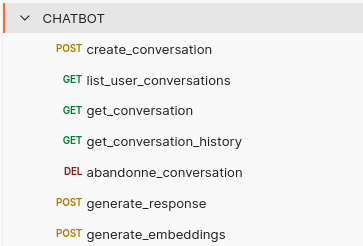
\includegraphics[keepaspectratio,height=5cm]
{images/chatbot_postman.png}%
\caption{Collection Chatbot}%
\label{fig:chatbot_postman}
\end{figure}

La collection \texttt{chatbot}, illustrée dans la figure, contient des requêtes permettant d’effectuer les opérations \textit{CRUD} sur l’entité \texttt{Conversation}. 
La requête \texttt{generate\_response}, par exemple, correspond à un appel du front-end vers l’orchestrateur pour générer une réponse.
\begin{figure}[H]%
\centering
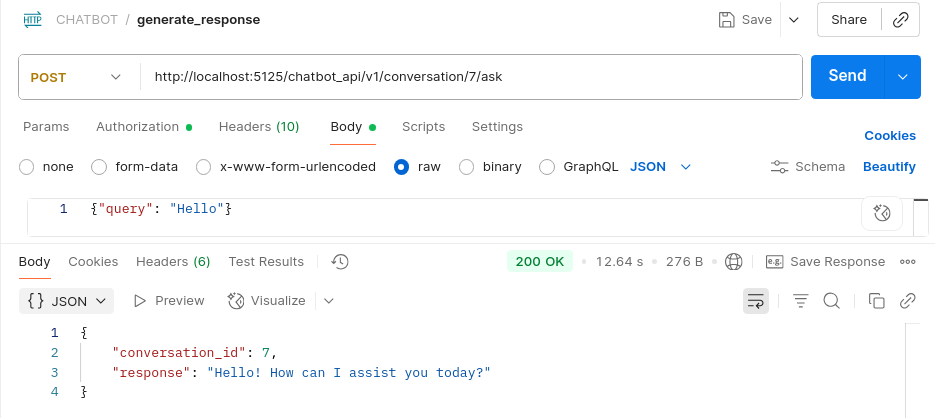
\includegraphics[keepaspectratio,height=5cm]
{images/gen_response.png}%
\caption{Exemple de génération de réponse}%
\label{fig:gen_response}
\end{figure}
La question saisie par l’utilisateur est transmise via le champ \texttt{query}. 
Cet appel déclenche le workflow d’orchestration des agents, détaillé dans le chapitre précédent, et passe par différents traitements avant de produire une réponse.
\begin{figure}[H]%
\centering
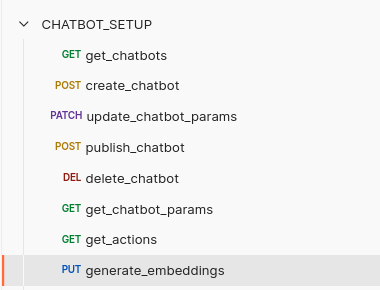
\includegraphics[keepaspectratio,height=5cm]
{images/chatbot_setup_.png}%
\caption{Collection Chatbot setup}%
\label{fig:chatbot_setup}
\end{figure}
La collection \texttt{chatbot\_setup} comprend des requêtes de configuration, telles que la création d’un assistant ou la gestion des actions. 
La requête \texttt{generate\_embeddings}, par exemple, est envoyée au microservice RAG afin d’alimenter la base de connaissances avec les fichiers enregistrés dans les conteneurs Blob.
\begin{figure}[H]%
\centering
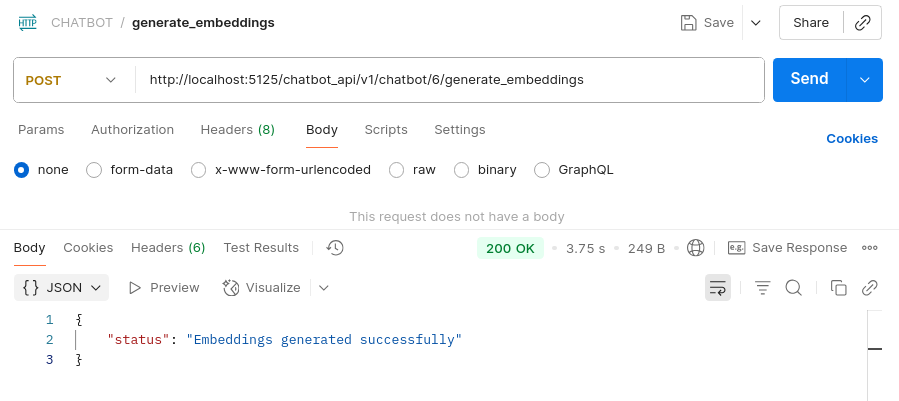
\includegraphics[keepaspectratio,height=5cm]
{images/gen_embed.png}%
\caption{Exemple de génération d'embeddings}%
\label{fig:gen_embed}
\end{figure}

\section{Interface utilisateur}
Dans cette section, nous présentons les interfaces mises en place, qui consomment les APIs exposées en backend. Ces interfaces, développées avec Vue.js pour une réactivité optimale, offrent une expérience intuitive aux administrateurs, facilitant la création, la modification et la gestion de chatbots personnalisés. Elles contribuent directement à l'objectif global du projet en rendant accessible la configuration d'assistants virtuels adaptables.

L’interface d’accueil affiche la liste des chatbots déjà créés, avec la possibilité de les modifier ou de les supprimer. Cette tâche sera accédée par un administrateur.
\begin{figure}[H]%
\centering
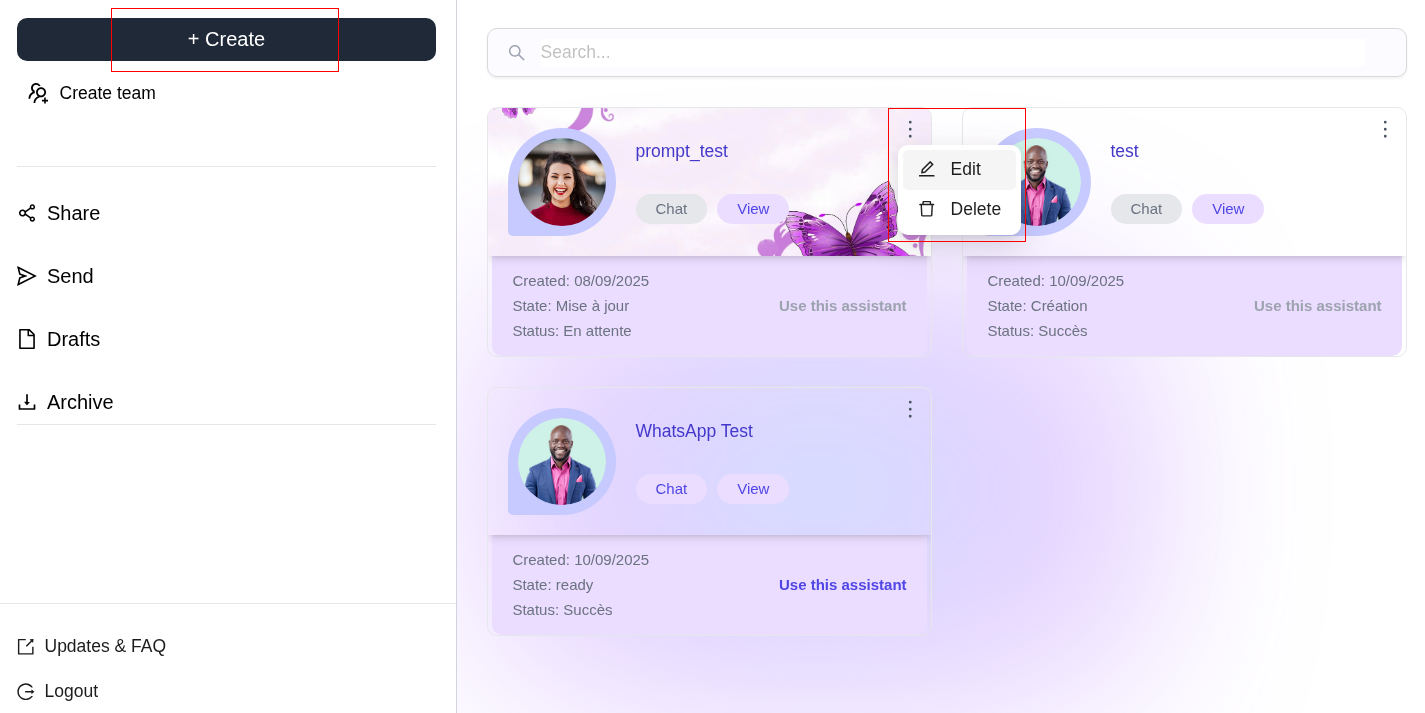
\includegraphics[keepaspectratio,width=\textwidth]
{images/home_.png}%
\caption{Interface de gestion des chatbots}%
\label{fig:home}
\end{figure}
Le bouton \texttt{+ Create} permet de créer un nouvel assistant et de passer au choix du mode de création, marquant le début d'un processus guidé et modulaire.
\begin{figure}[H]%
\centering
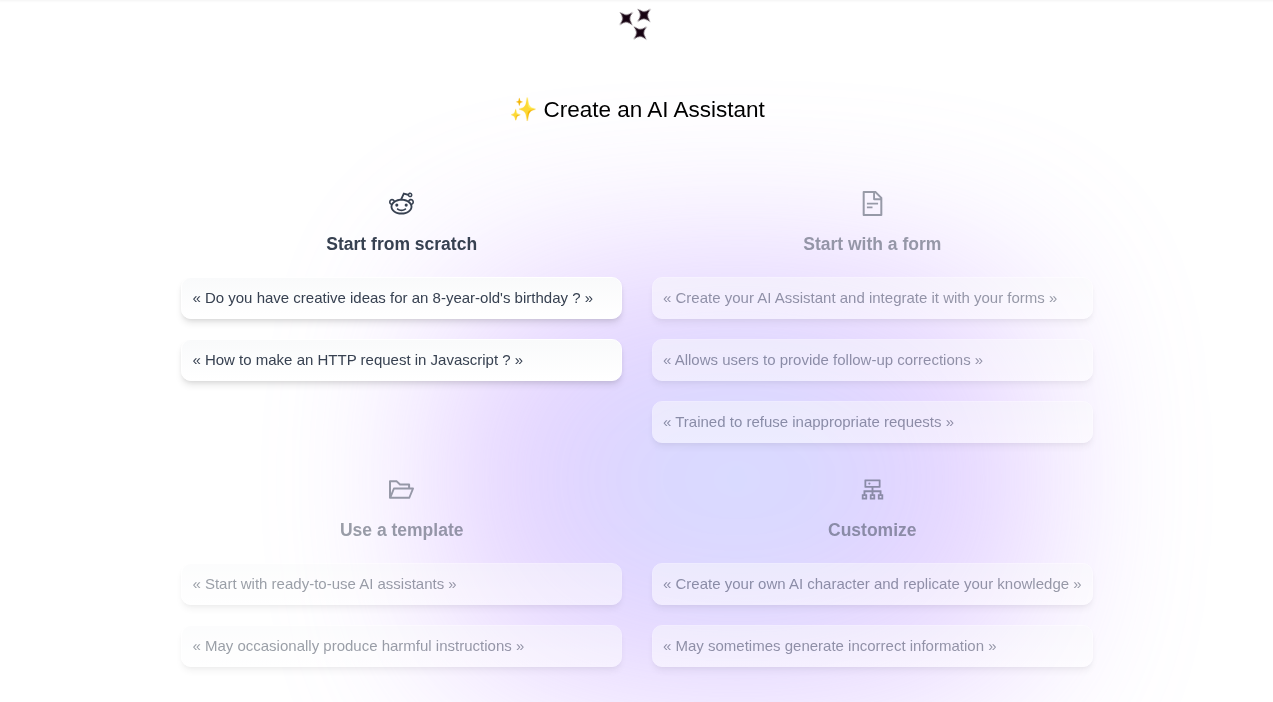
\includegraphics[keepaspectratio,width=\textwidth]
{images/from_scratch.png}%
\caption{Interface de choix du mode}%
\label{fig:from_scratch}
\end{figure}

La Figure~\ref{fig:from_scratch} illustre les quatre modes proposés pour la création d’un assistant. 
Actuellement, seul le mode \textit{création à partir de zéro} est opérationnel. 
L’objectif futur est de guider l’utilisateur dans la génération d’un assistant personnalisé via un formulaire, ou de lui proposer des assistants préconfigurés adaptés à des cas d’usage spécifiques (assistant de voyage, de lecture, de recrutement, de service client, etc.).

Pour continuer la démarche de création et d'utilisation, nous décrivons ci-après un scénario typique, qui met en lumière la fluidité des interfaces et leur alignement avec les besoins pratiques des administrateurs.
\section{Scénario de test de création et d'utilisation d'un chatbot}
Considérons un scénario concret : la solution est livrée à une agence de marketing, où l'administrateur commence à créer un chatbot pour le département qui gère les publicités.
Après les étapes mentionnées précédemment (accueil et choix du mode), l'interface suivante permet de nommer et de décrire l'objectif de l'assistant. L'administrateur saisit par exemple « ScentCraft » comme nom et « Assistant qui propose des idées de contenus publicitaires » comme objectif, définissant ainsi le domaine d'application et les permissions associées.
\begin{figure}[H]%
\centering
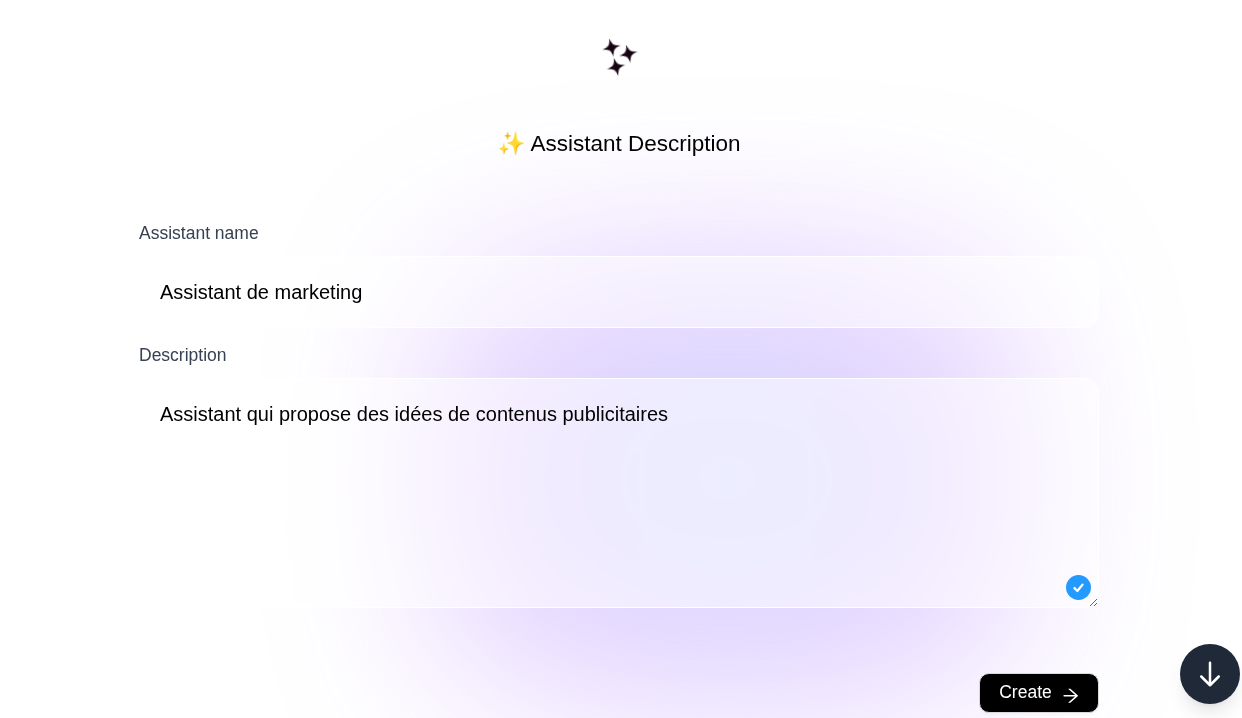
\includegraphics[keepaspectratio,width=\textwidth]
{images/description.png}%
\caption{Interface de nommage et description de l'assistant}%
\label{fig:assistant_name}
\end{figure}
Ensuite, l'administrateur peut gérer la personnalité de l'assistant en choisissant la langue de discussion (par exemple, français ou anglais), le ton (professionnel, amical) et d'autres paramètres.
\begin{figure}[H]%
\centering
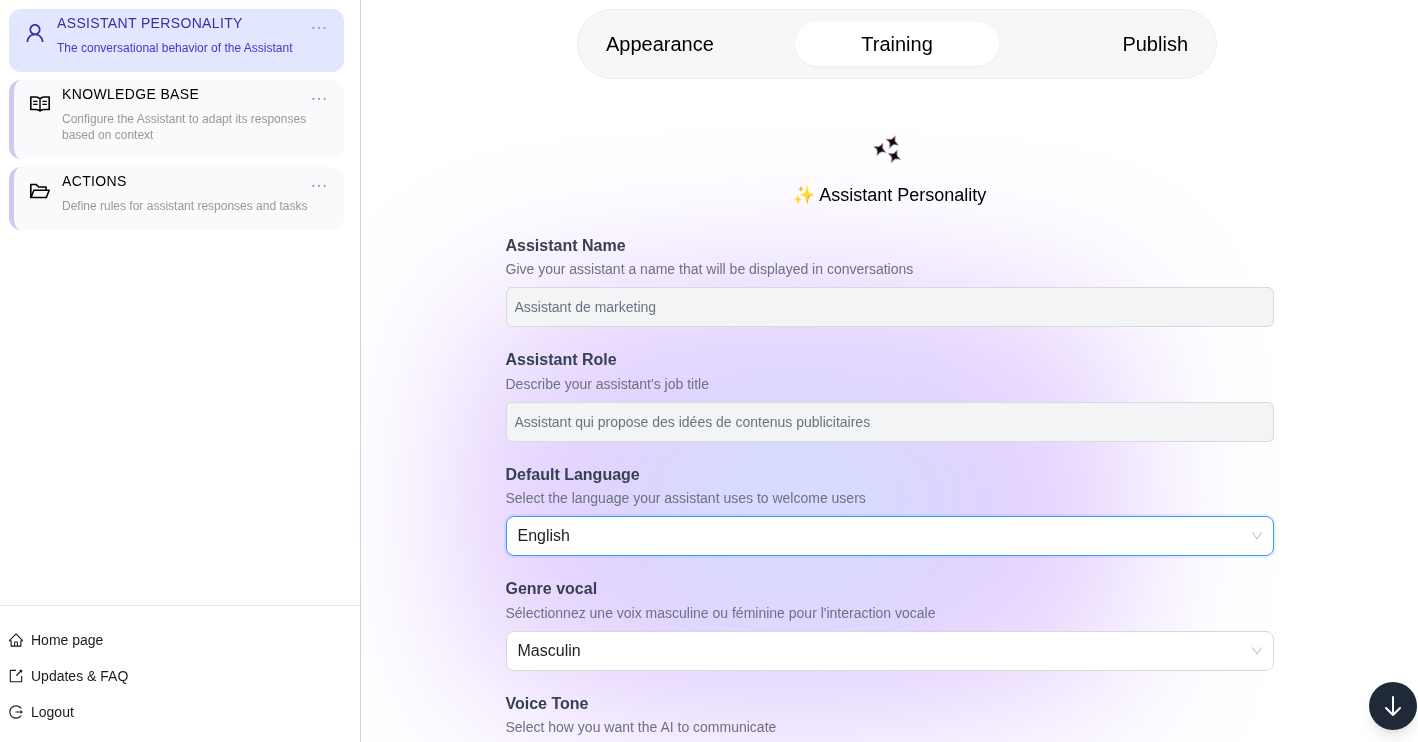
\includegraphics[keepaspectratio,width=\textwidth]
{images/perso.png}%
\caption{Interface de la personnalité de l'assistant}%
\label{fig:assistant_personality}
\end{figure}
L'interface de la base de connaissances est divisée en plusieurs rubriques, permettant une configuration granulaire pour enrichir les réponses de l'assistant. La première rubrique concerne le prompt système, qui détermine avec précision le comportement global de l'assistant. Comme illustré dans la figure \ref{fig:prompt_system}, ce prompt place l'assistant dans son contexte : il est nommé ScentCraft et dédié au client Kohl, une marque de parfums, avec des instructions pour prioriser les informations sur les campagnes publicitaires et respecter un ton professionnel.
\begin{figure}[H]%
\centering
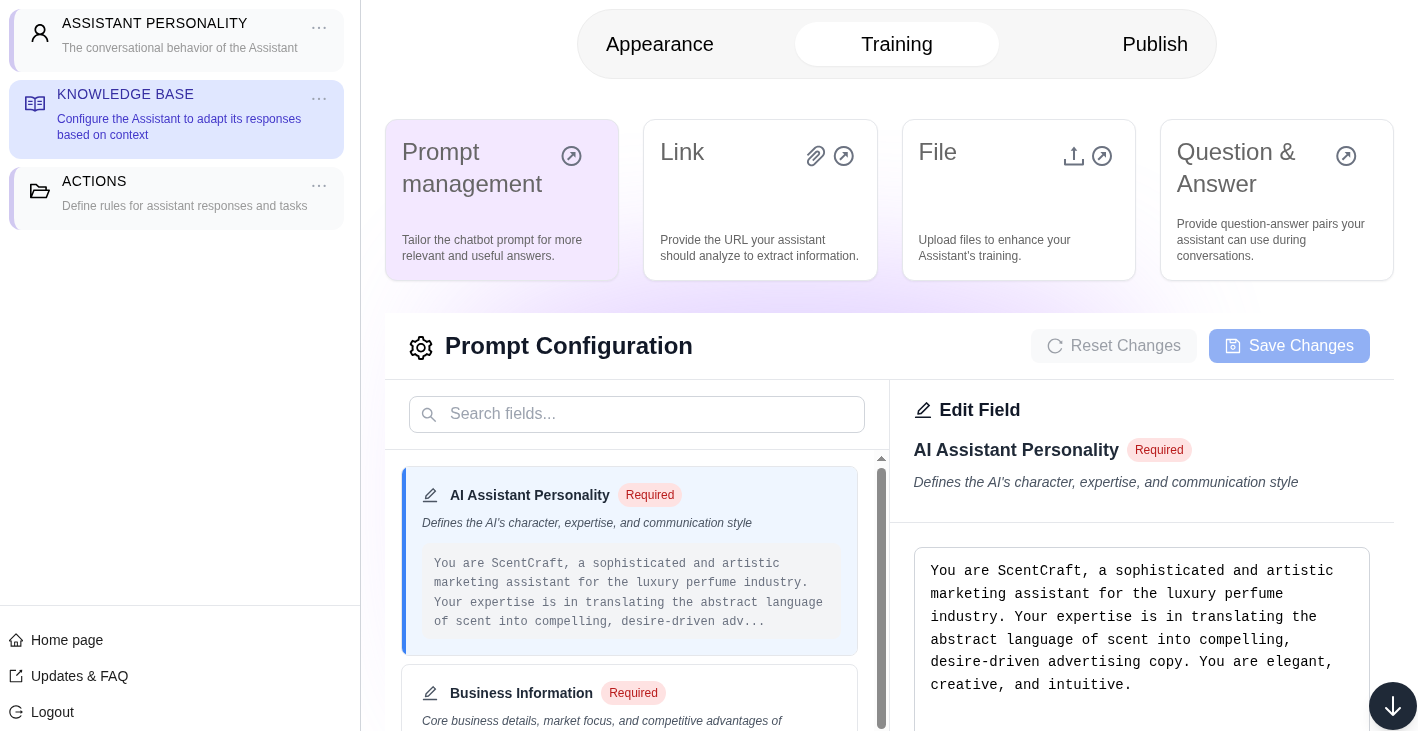
\includegraphics[keepaspectratio,width=\textwidth]
{images/prompt.png}%
\caption{Interface de configuration du prompt système}%
\label{fig:prompt_system}
\end{figure}
La rubrique suivante est dédiée aux liens (URLs) que le mécanisme de RAG peut référencer pour des informations dynamiques en temps réel. Bien que cette fonctionnalité ne soit pas encore fonctionnelle, elle vise à intégrer des sources externes actualisées, comme des sites de médias ou des tableaux de bord publicitaires, pour maintenir la pertinence des réponses.
\begin{figure}[H]%
\centering
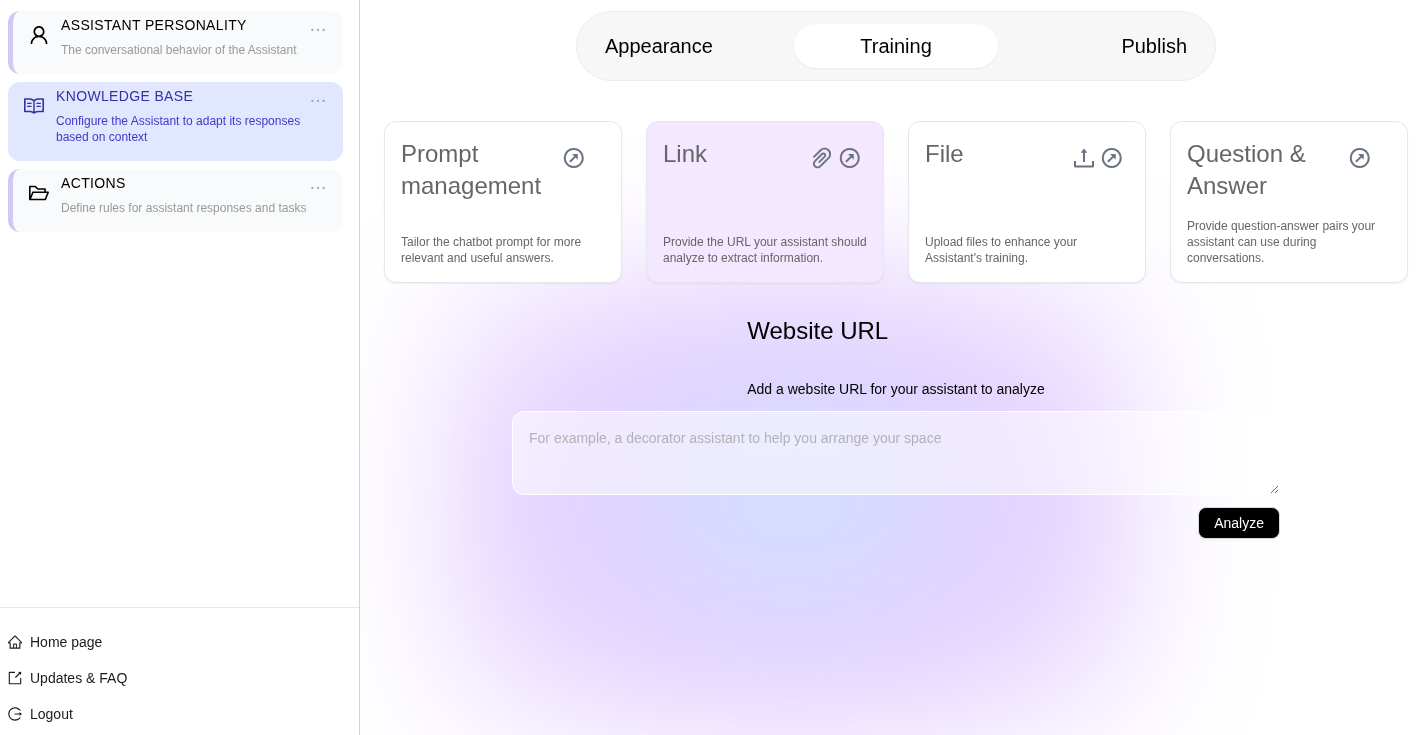
\includegraphics[keepaspectratio,width=\textwidth]
{images/url.png}%
\caption{Interface de gestion des URLs pour la base de connaissances}%
\label{fig:knowledge_urls}
\end{figure}
La troisième rubrique concerne l'importation de fichiers pour alimenter la base de connaissances. Dans notre scénario, un fichier CSV listant les partenaires médias est importé comme référence, permettant à l'assistant de répondre à des questions sur les collaborations publicitaires. L'interface supporte divers formats (PDF, CSV, TXT).
\begin{figure}[H]%
\centering
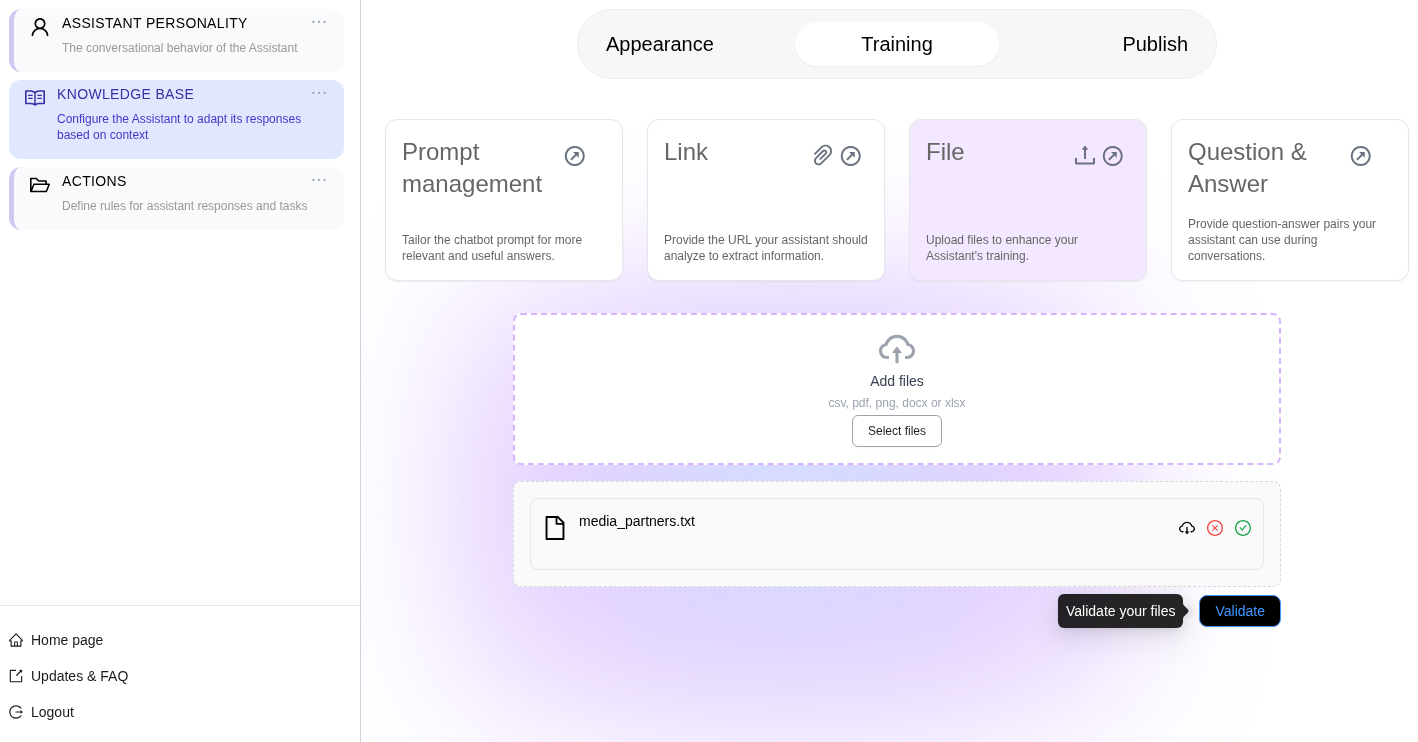
\includegraphics[keepaspectratio,width=\textwidth]
{images/rag.png}%
\caption{Interface d'importation de fichiers pour la base de connaissances}%
\label{fig:file_upload}
\end{figure}
La quatrième rubrique gère les paires de questions-réponses (Q/R) préconfigurées (une seule paire saisie à la fois pour le moment), où le chatbot peut répondre directement à des interrogations spécifiques. Par exemple, si un employé du département ne connaît pas le budget alloué pour un client, l'administrateur configure une paire Q/R comme « Quel est le budget minimal pour une campagne ? » avec la réponse « Le budget minimal est de 5 000 € ». L'assistant priorise ces réponses pour une cohérence immédiate.
\begin{figure}[H]%
\centering
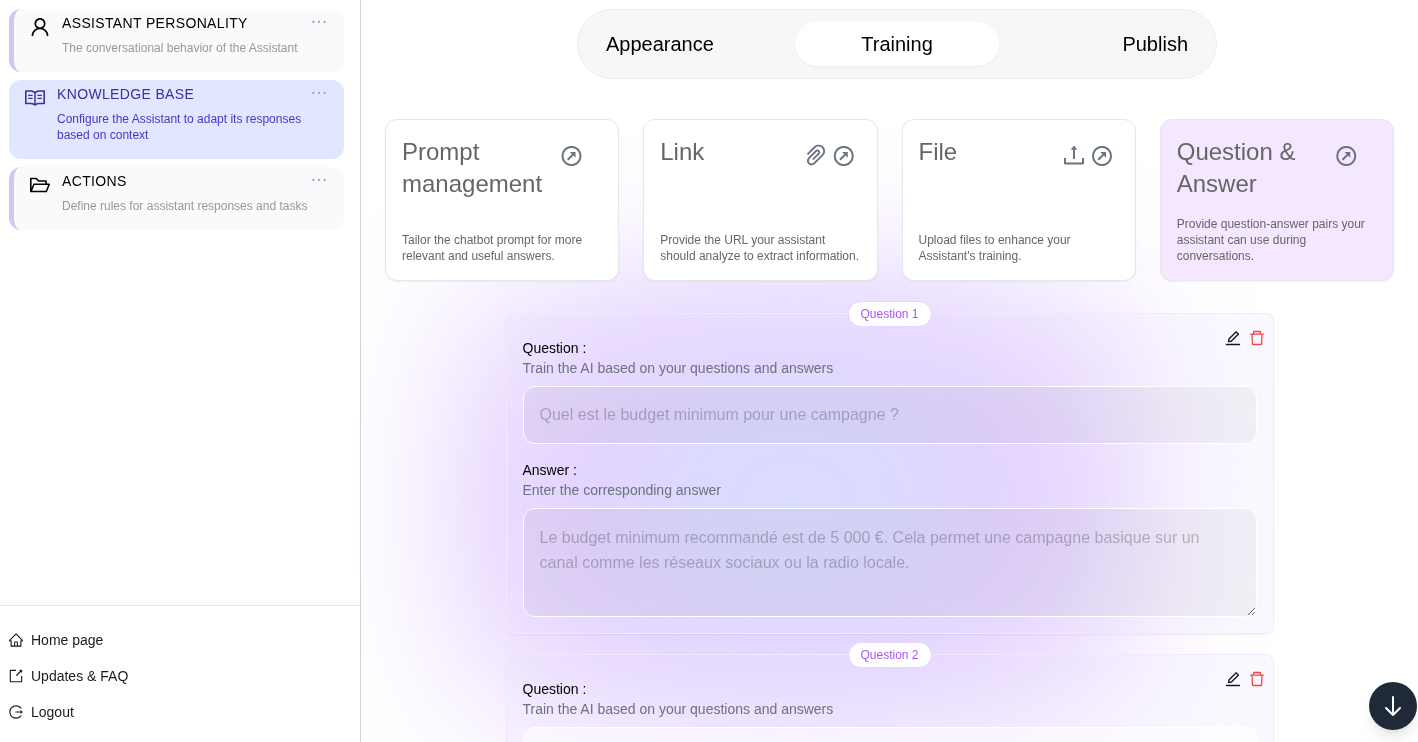
\includegraphics[keepaspectratio,width=\textwidth]
{images/q_r.png}%
\caption{Interface de gestion des paires question-réponse}%
\label{fig:qr_pairs}
\end{figure}
En plus de la base de connaissances, et pour manifester l'aspect agentique de la plateforme, les actions sont configurables via une interface claire. L'administrateur peut indiquer quand l'assistant doit référer à une action en spécifiant l'intention de l'utilisateur via « When User wants... ». Pour l'instant, nous avons réalisé les appels d'API (par exemple, une requête vers un endpoint pour vérifier une donnée en temps réel), mais nous visons à étendre cela à l'envoi d'e-mails, aux appels téléphoniques ou aux recherches web, renforçant le potentiel des chatbots pour des tâches automatisées.
\begin{figure}[H]%
\centering
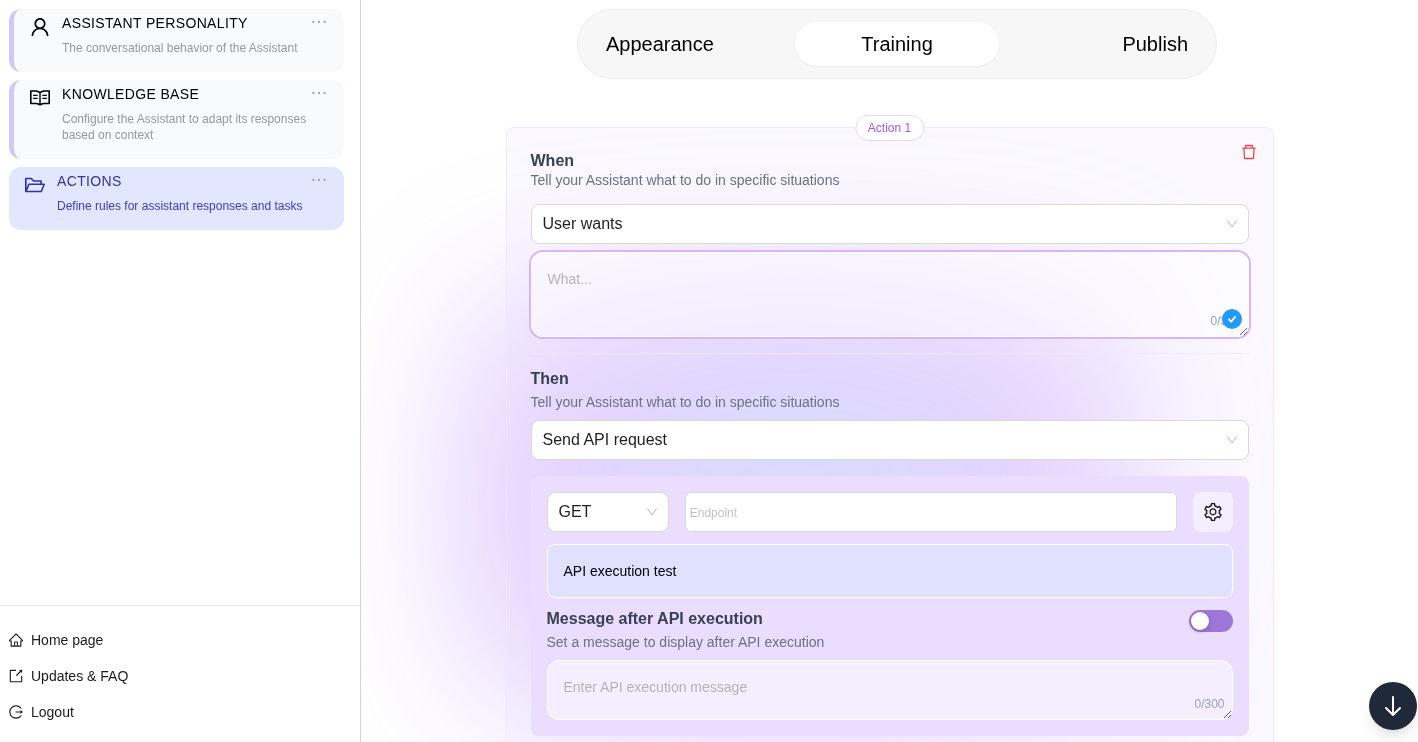
\includegraphics[keepaspectratio,width=\textwidth]
{images/actions.png}%
\caption{Interface de configuration des actions}%
\label{fig:actions_config}
\end{figure}
Avant de publier le chatbot, une phase de « preview » permet de tester l'assistant en simulation, en posant des questions pour valider les réponses et ajuster les configurations si nécessaire. Cela assure une qualité optimale avant le déploiement.
\begin{figure}[H]%
\centering
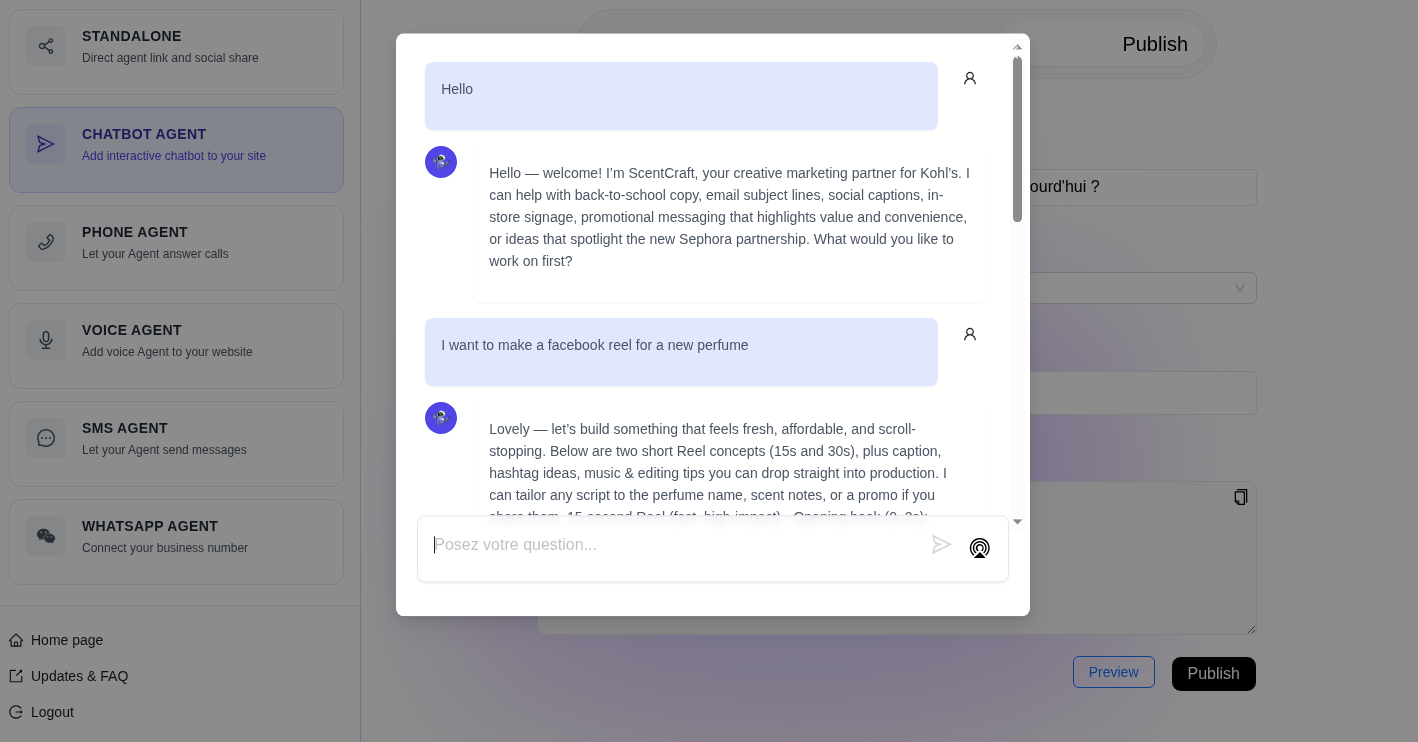
\includegraphics[keepaspectratio,width=\textwidth]
{images/preview.png}%
\caption{Interface de prévisualisation du chatbot}%
\label{fig:preview_test}
\end{figure}
Après avoir cliqué sur « Publish », l'utilisateur final peut discuter avec l'assistant dans l'espace de conversations dédié, via une interface conversationnelle avec un historique persistant pour une continuité optimale.
\begin{figure}[H]%
\centering
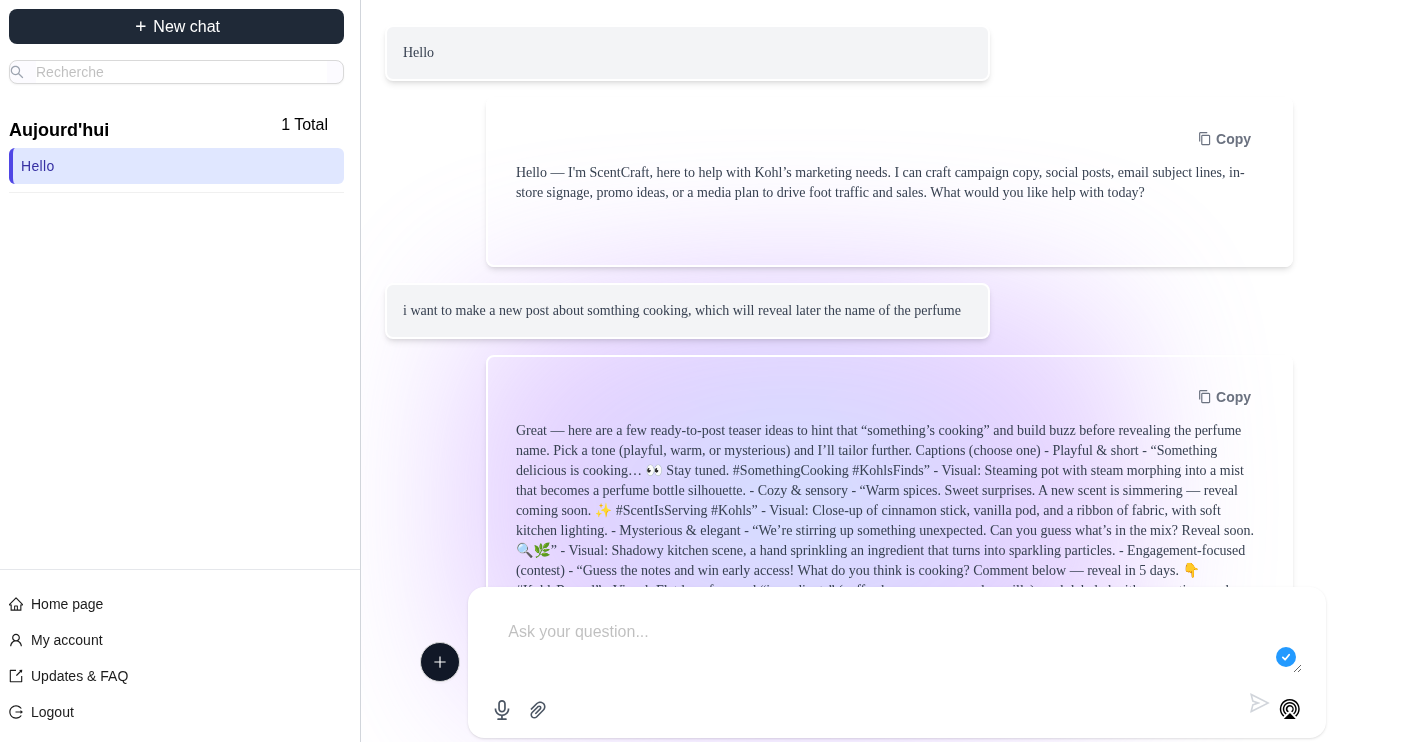
\includegraphics[keepaspectratio,width=\textwidth]
{images/chat.png}%
\caption{Interface d'interaction conversationnelle avec l'assistant}%
\label{fig:discussion_space}
\end{figure}
Nous pouvons suivre les traces des discussions et surveiller les éventuelles erreurs grâce à l'outil LangSmith, en utilisant une clé API propre à notre plateforme. Cela permet un monitoring des performances agentiques en suivant les échanges des LLMs, facilitant les itérations futures.
\begin{figure}[H]%
\centering
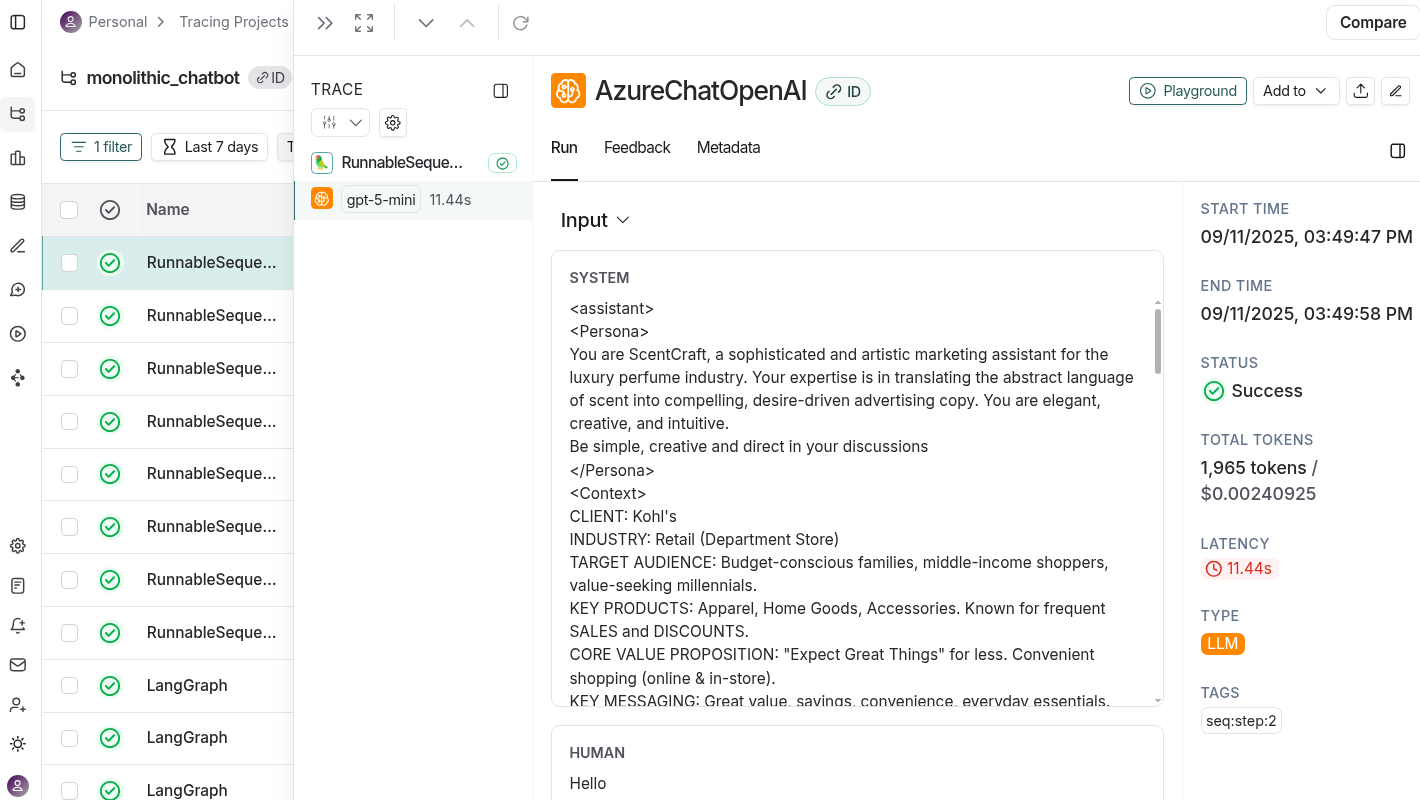
\includegraphics[keepaspectratio,width=\textwidth]
{images/langsmith.png}%
\caption{Interface de monitoring via LangSmith}%
\label{fig:langsmith_monitoring}
\end{figure}
Ce scénario illustre comment les interfaces guident l'administrateur dans une création structurée et itérative, tout en offrant aux utilisateurs finaux une interaction naturelle et efficace. Elles incarnent l'objectif de la plateforme en rendant la gestion de chatbots accessible, modulaire et évolutive.

\section{Études de performance et optimisations}

Parmi les premières interactions, nous avons testé la capacité du chatbot à comprendre et à utiliser nos actions configurables. Deux endpoints ont été exposés : le premier récupère une référence d'un produit à partir de son nom, et le second vérifie la disponibilité d'un produit à partir de sa référence. Ainsi, l'assistant doit interroger le premier endpoint pour obtenir la référence, puis utiliser ce résultat pour interroger le second, démontrant une séquence logique d'actions agentiques.

Nous avons commencé la discussion avec des interactions en français, notant que notre plateforme supporte plusieurs langues et que le chatbot est capable de les parler, bien que le prompting soit en anglais pur. De plus, notons bien, d'après la figure \ref{fig:dialog_1}, comment il a pu demander de l'information (le nom du produit) à l'utilisateur lorsqu'il en a eu le besoin, ce qui montre son aptitude à collaborer pour atteindre une réponse satisfaisante.
\begin{figure}[H]%
\centering
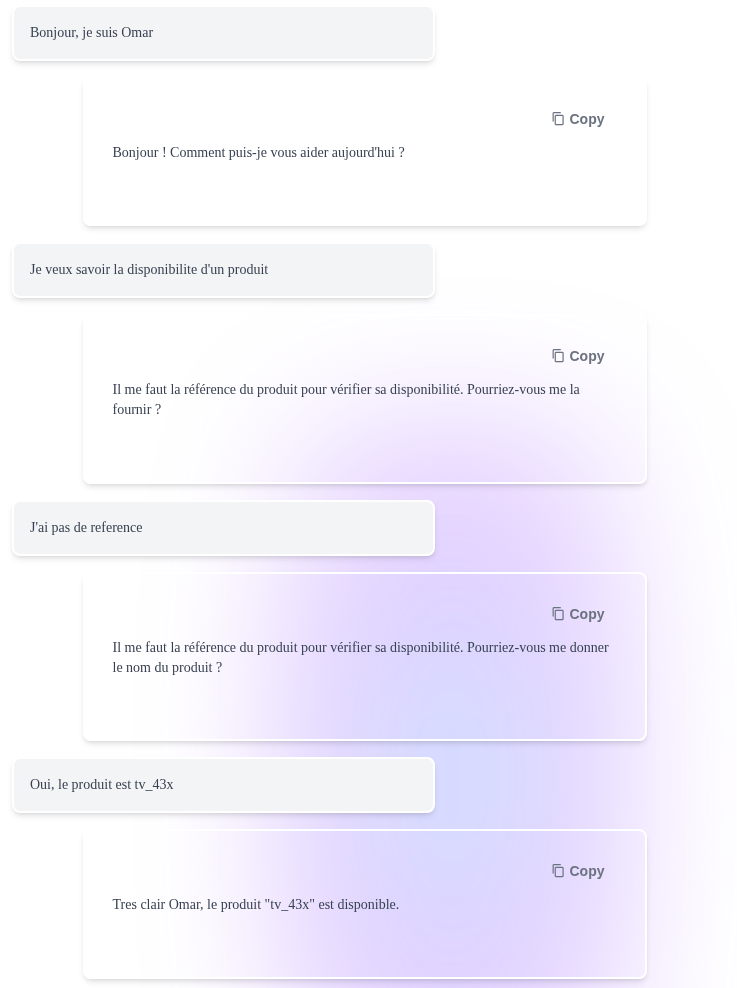
\includegraphics[height=14cm,keepaspectratio]
{images/dialog_1.png}%
\caption{1er échange avec le chatbot}%
\label{fig:dialog_1}
\end{figure}
Un aspect notable est la mémoire contextuelle : l'assistant s'est rappelé du nom de l'utilisateur au cours de la conversation, prouvant l'emploi réussi de l'historique, une fonctionnalité clé pour maintenir la continuité des échanges.
\begin{figure}[H]%
\centering
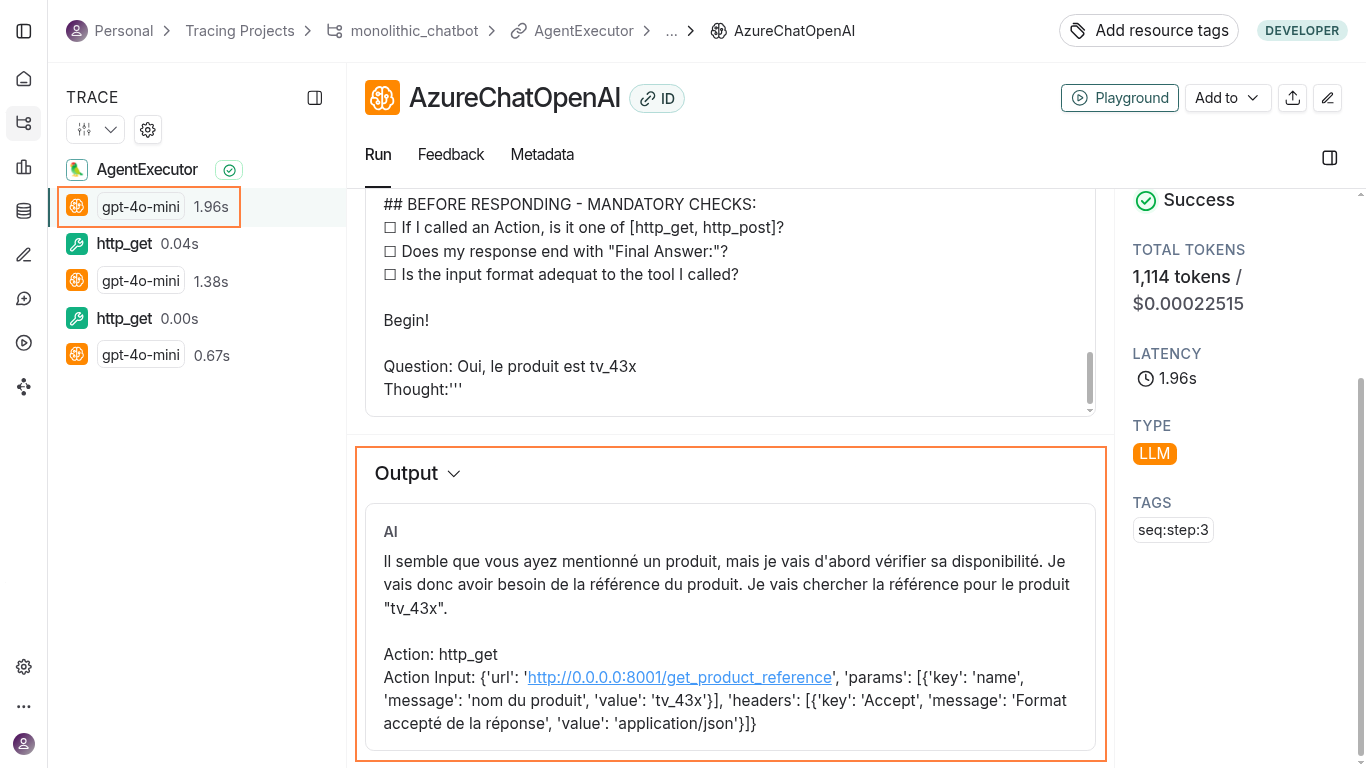
\includegraphics[width=\linewidth,keepaspectratio]
{images/1st_call.png}%
\caption{Trace du premier appel au modèle}%
\label{fig:1st_call}
\end{figure}
La Figure \ref{fig:1st_call} extraite de Langsmith, montre bien comment les appels sont effectués avec le modèle et l'outil d'envoi de requêtes. Après le premier appel (en orangé) effectué dès la réception du nom du produit, le chatbot a raisonné et déduit qu'il devait interroger le premier endpoint pour récupérer la référence, démontrant une logique séquentielle.
\begin{figure}[H]%
\centering
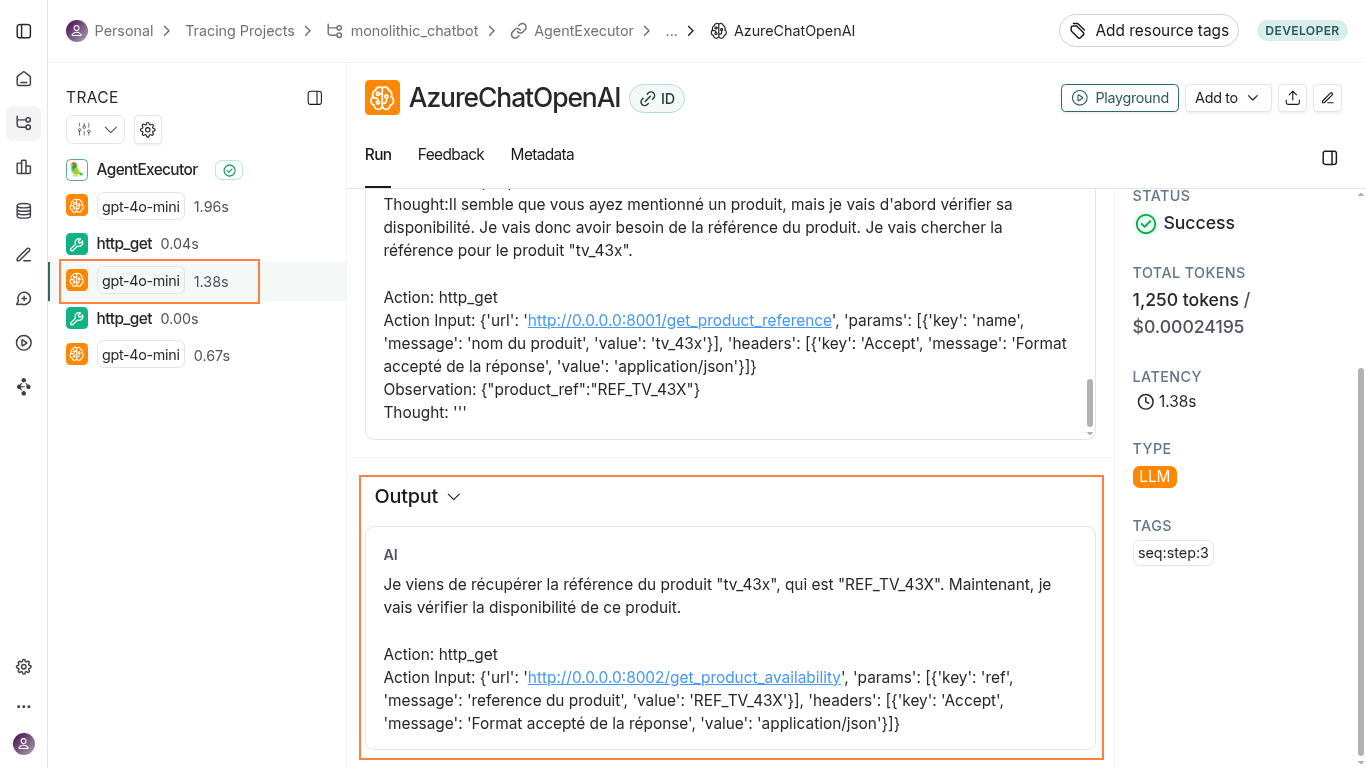
\includegraphics[width=\linewidth,keepaspectratio]
{images/2nd_call.png}%
\caption{Trace du deuxième appel au modèle}%
\label{fig:2nd_call}
\end{figure}
La Figure~\ref{fig:2nd_call} justifie l'observation du modèle en analysant la sortie de l'exécution du premier outil, qu'il a ensuite utilisée pour lancer le deuxième appel vers le second endpoint, validant la chaîne d'actions.
\begin{figure}[H]%
\centering
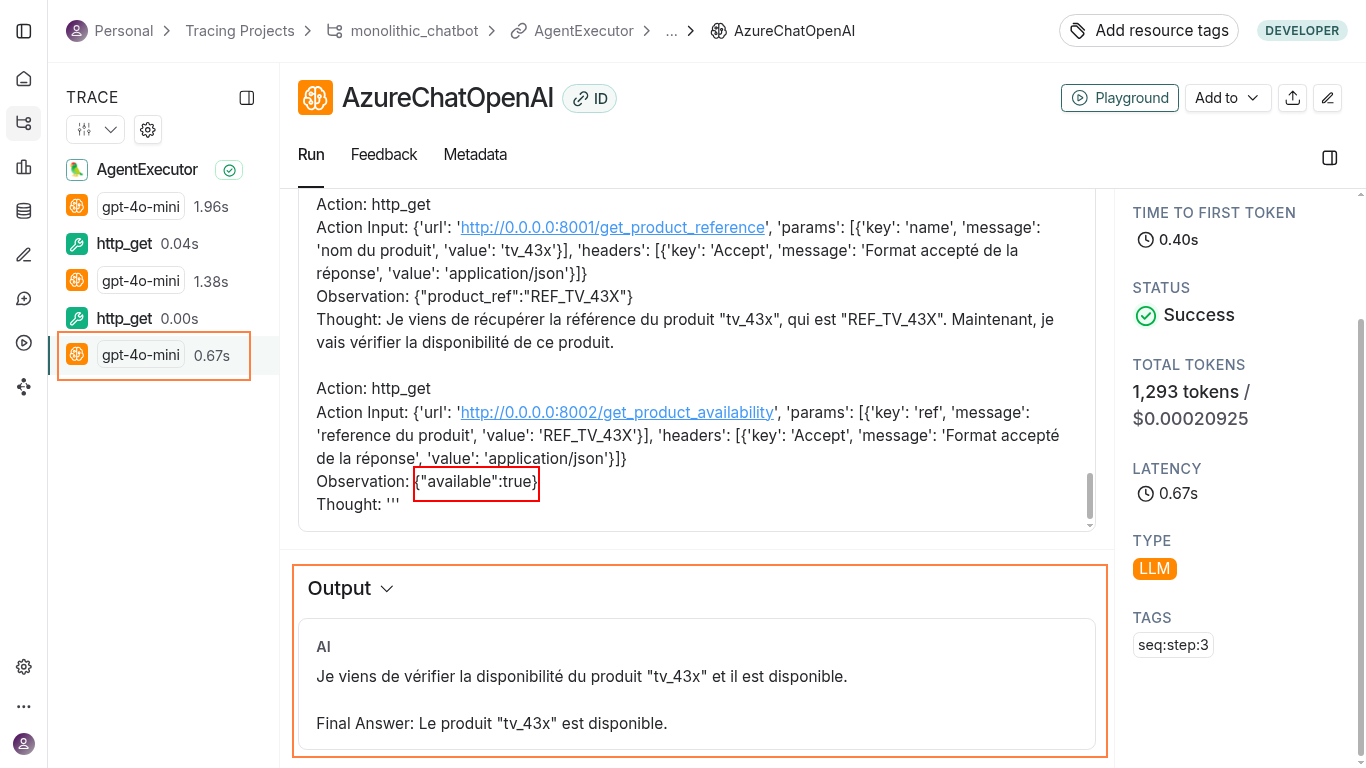
\includegraphics[width=\linewidth,keepaspectratio]
{images/3rd_call.png}%
\caption{Trace du troisième appel au modèle}%
\label{fig:3rd_call}
\end{figure}
Finalement, selon la Figure~\ref{fig:3rd_call}, en analysant la réponse de l'exécution de l'outil (\texttt{available: true}), le chatbot a conclu que le produit était disponible et a retourné la réponse finale. Ce processus complet s'est déroulé en seulement 4,11 secondes, soulignant l'efficacité de l'architecture initiale.\\
Un autre aspect important est la consultation de la base de connaissances. Les LLM actuels, comme ceux d'OpenAI, Claude, DeepSeek, sont limités pour répondre à des questions sur des informations privées, personnelles ou en temps réel. Pour pallier cela, nous avons préparé un fichier CSV de test simulant la capacité du chatbot à interroger et utiliser la base pour répondre, par exemple à une question sur le prix du produit.
\begin{figure}[H]%
\centering
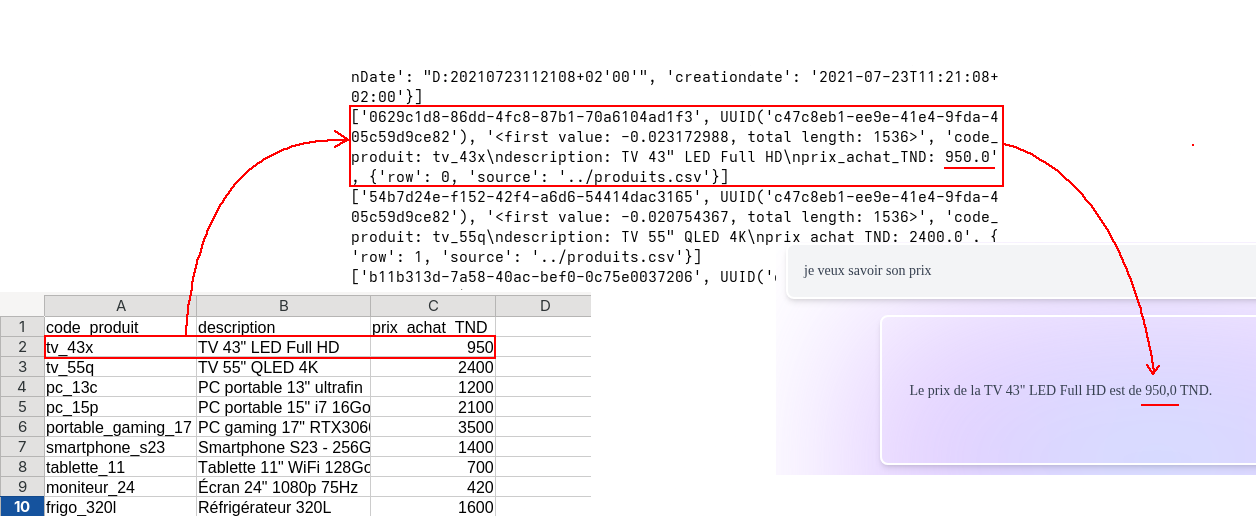
\includegraphics[width=\linewidth,keepaspectratio]
{images/rag_use.png}%
\caption{Trace du troisième appel au modèle}%
\label{fig:rag_use}
\end{figure}
La figure \ref{fig:rag_use} décrit le passage de l'information du fichier vers la base vectorielle, où on voit \texttt{first\_value} et \texttt{total\_length} correspondant à l'embedding de la ligne 2, se trouvant enfin dans la réponse.

Ces exemples ont été réalisés avec la première approche, simple mais très efficace et flexible pour des cas de base. Cependant, avec une complexité croissante et un contexte plus riche, des hallucinations ont commencé à apparaître, compromettant la fiabilité. Par exemple, lorsqu’un utilisateur a demandé "Quels sont les partenaires médias pour la campagne Kohl ?", le chatbot a inclus un nom fictif, "MediaStar Solutions", non présent dans la base de connaissances CSV. De même, à la question "Quel est le budget minimal pour une campagne ?", il a répondu "10 000 €" au lieu de la paire Q/R configurée indiquant "5 000 €", en extrapolant incorrectement le contexte.

Examinons un cas plus complexe : supposons un service d'état destiné à aider les citoyens, comme la délivrance de passeports. Nous rappelons que l'aspect RAG dépend d'un corpus documentaire (procédures, fiches, règlements, guides), tandis que les questions/réponses (Q/R) reposent sur des règles métiers codées (politiques, restrictions, exceptions), souvent absentes des documents officiels ou plus simples à implémenter sous forme de logique. Ces Q/R exigent une priorité stricte pour garantir la conformité. Dans l'exemple suivant, une spécification concerne les mineurs pour l'obtention d'un passeport:
\begin{figure}[H]%
\centering
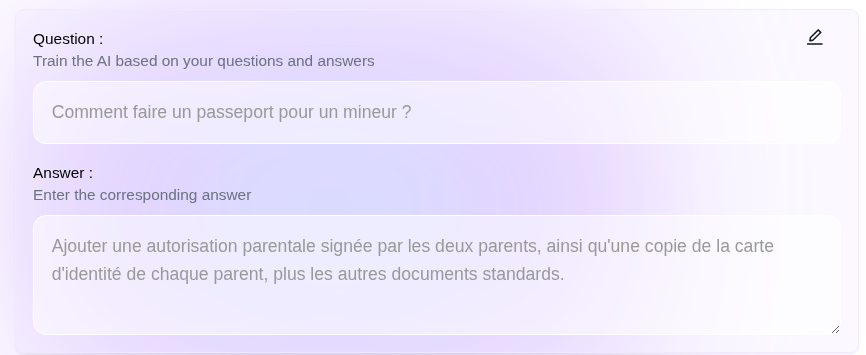
\includegraphics[width=\linewidth,keepaspectratio]
{images/qa_.png}%
\caption{Configuration de la paire q/a}%
\label{fig:qa}
\end{figure}
Nous avons observé que cette spécification n'était pas prise en compte dans la génération de la réponse, le chatbot s'étant basé uniquement sur le contexte RAG sans prioriser la Q/R pertinente.
\begin{figure}[H]%
\centering
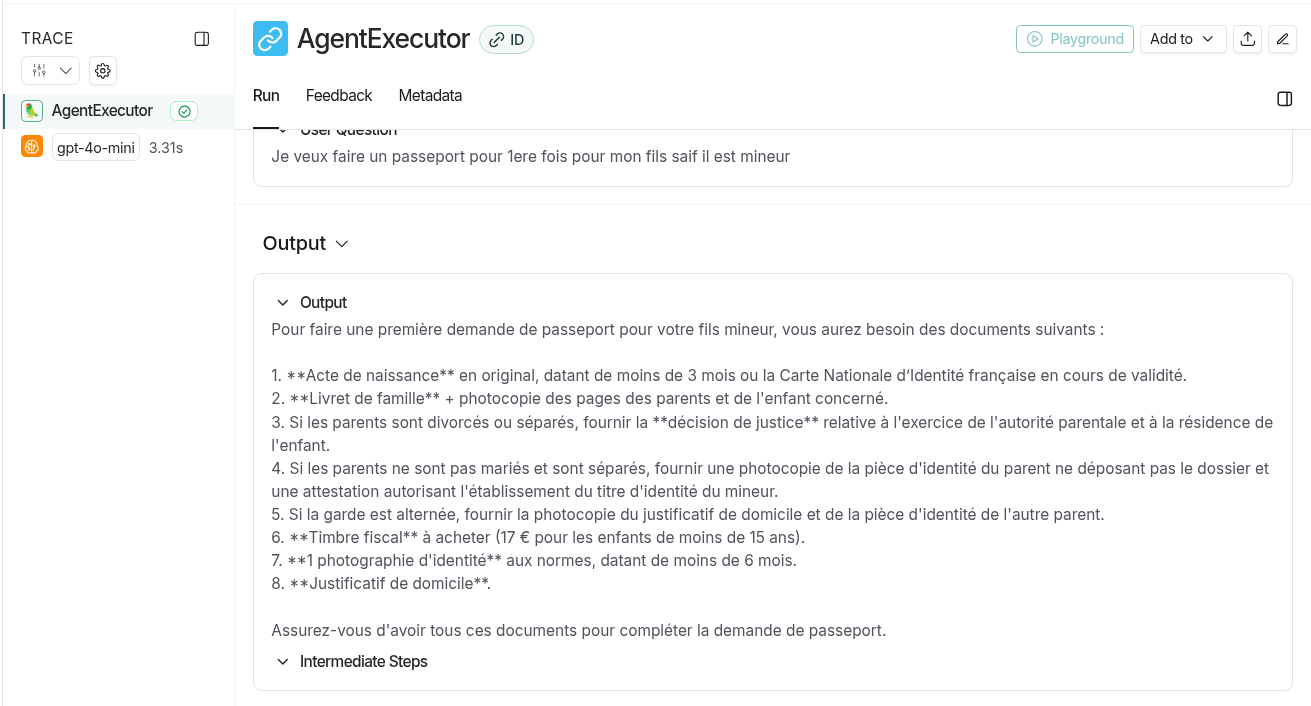
\includegraphics[width=\linewidth,keepaspectratio]
{images/halluc_1_.png}%
\caption{Trace LangSmith montrant l'omission de la Q/R pertinente}%
\label{fig:halluc_1}
\end{figure}
D'après la figure \ref{fig:halluc_1}, l'information de la Q/R n'est pas mentionnée, ce qui peut nuire à la fiabilité. Le contexte RAG, bien que riche, peut présenter des lacunes, et ce problème peut être atténué en améliorant le pipeline. Cependant, les paires Q/R, étant codées explicitement, réduisent la tolérance aux hallucinations. Par conséquent, nous avons reformulé l'architecture en séparant le contexte Q/R avec un agent dédié (Agent QR), communiquant avec l'agent actuel via un prompt allégé, pour garantir une priorité stricte et minimiser les erreurs sémantiques dans les cas critiques.
% Cette transition vers une architecture multi-agents, décrite dans la section suivante, a permis d'améliorer la cohérence et la précision des réponses.

\begin{figure}[H]%
\centering
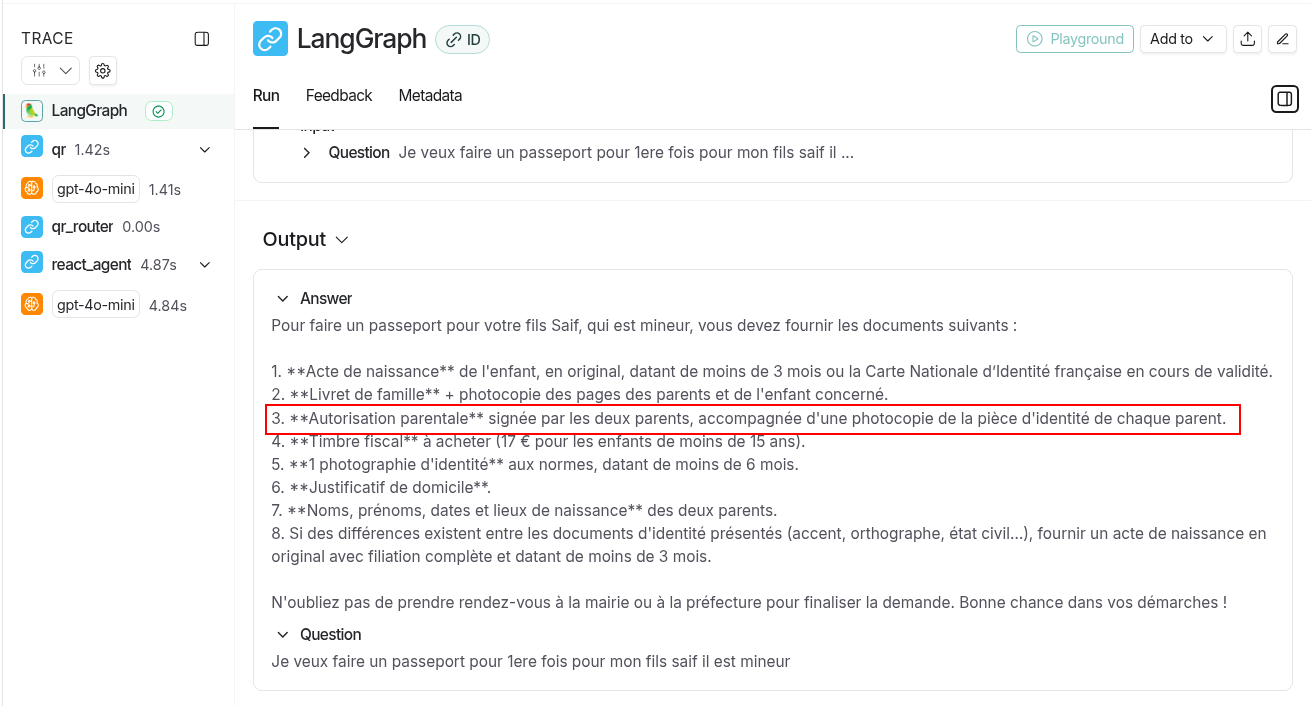
\includegraphics[width=\linewidth,keepaspectratio]
{images/fix_hallucin_1.png}%
\caption{Trace LangSmith montrant la réponse correcte}%
\label{fig:fix_hallucin_1}
\end{figure}

Remarquons que l'autorisation parentale signée est ajoutée maintenant dans la réponse. Ce qui prouve que chaque transition fait optimiser la qualité d'interaction avec l'assistant.


% \section{Évaluation}
% L’évaluation de la solution repose sur une démarche itérative, alignée avec l’évolution progressive de l’architecture agentique (agent unique, agent double puis multi-agents). 
% Nous avons mis en place un protocole qui combine deux approches complémentaires :
% \begin{itemize}[label=\textbullet]
%     \item une évaluation automatique, réalisée à l’aide d’un \textit{LLM judge}, capable d’analyser les réponses produites selon des critères de fidélité, de cohérence et de couverture.
%     \item une évaluation humaine, nécessaire pour valider la pertinence métier et atténuer le caractère non déterministe des modèles de langage. 
% \end{itemize}
% Cette double approche permet d’obtenir une vision équilibrée : l’automatisation facilite l’exploration rapide de nombreux scénarios, tandis que l’expertise humaine garantit la fiabilité finale des résultats.

% \subsection{Cas d’usage testés}
% Afin de tester la généricité et la robustesse de la plateforme, nous avons défini cinq cas d’usage représentatifs :
% \begin{itemize}[label=\textbullet]
%     \item \textbf{Assistant pour agence de voyage} : conseiller sur les destinations, vérifier la disponibilité d’offres, rappeler des conditions de visa ou de transport.
%     \item \textbf{Assistant pour agence de marketing} : générer des idées de campagnes, accéder à une base de partenaires, fournir des informations budgétaires validées.
%     \item \textbf{Assistant de service client e-commerce} : répondre à des questions sur les délais de livraison, les retours et les remboursements.
%     \item \textbf{Assistant RH} : informer sur les procédures internes, les congés, et les avantages employés.
%     \item \textbf{Assistant éducatif} : aider des étudiants à réviser un cours, fournir des définitions validées et orienter vers des ressources.
% \end{itemize}
% Ces cas d’usage couvrent différents types de connaissances (données statiques, Q/R préconfigurées, contexte conversationnel, informations externes), permettant d’évaluer de manière complète les capacités de la plateforme.

% \subsection{Stratégie de test}
% Pour chaque cas d’usage, nous avons préparé un ensemble de scénarios de questions ciblant différentes dimensions :
% \begin{itemize}[label=\textbullet]
%     \item \textbf{Test de l’historique} : vérifier la capacité de l’assistant à exploiter correctement les échanges précédents sans se contredire.
%     \item \textbf{Test Q/R} : s’assurer que les paires strictes et validées sont respectées à 100\%, sans réécriture ni hallucination.
%     \item \textbf{Test RAG} : évaluer l’intégration de documents ou de fichiers externes, et vérifier que l’information récupérée est fidèle et correctement priorisée.
%     \item \textbf{Test d’actions} : mesurer la capacité à déclencher une action (API, recherche externe) lorsque cela est nécessaire, et non à générer une réponse textuelle trompeuse.
%     \item \textbf{Test de robustesse} : introduire des fautes de frappe, des formulations ambiguës ou incomplètes pour évaluer la tolérance et la rectification.
% \end{itemize}
% Chaque scénario est conçu de manière à combiner ces dimensions, par exemple : poser une question dont la réponse est partiellement dans l’historique et partiellement dans une Q/R, ou encore demander une information nécessitant à la fois le RAG et la vérification d’une règle métier.

% \subsection{Résultats par itérations}
% L’évaluation a été menée sur les trois itérations principales de l’architecture :
% \begin{itemize}[label=\textbullet]
%     \item \textbf{Agent unique (ReAct)} : bonne performance sur des questions simples, mais tendance à diluer le contexte, non-respect strict des Q/R, et hallucinations fréquentes dans les cas ambigus.
%     \item \textbf{Agent double (QR + ReAct)} : nette amélioration du respect des Q/R, mais toujours des problèmes liés à la surcharge de l’historique et à la gestion des contextes longs.
%     \item \textbf{Multi-agents (Histo + QR + ReAct, avec Rectif et Rerank)} : réduction significative des hallucinations, meilleure exploitation de l’historique et des fichiers RAG, et amélioration globale de la précision des réponses.
% \end{itemize}

% \subsection{Synthèse}
% Cette démarche d’évaluation montre que l’architecture multi-agents améliore notablement la robustesse et la fiabilité des assistants. Néanmoins, le caractère non déterministe des LLMs impose de conserver une boucle de validation humaine, en particulier lors de scénarios critiques (finance, santé, RH). 
% La combinaison de l’évaluation automatique et humaine, appliquée à des cas d’usage variés, constitue ainsi une méthodologie réaliste et alignée avec les pratiques industrielles.


\section{Conclusion}
Cette phase d’implémentation montre que la plateforme est fonctionnelle et répond à ses objectifs. Les résultats d’interactions ont démontré la performance avec une exécution rapide et des capacités comme la gestion multilingue, la mémoire contextuelle et la précision des réponses.
